\documentclass{report}
\usepackage[utf8]{inputenc}
\usepackage{multicol}
\usepackage{geometry}
\usepackage{graphicx}
\usepackage{spf}
\usepackage{comment}
\geometry{top=3cm, bottom=3cm, left=2cm, right=2cm}
\title{Sous une pluie de feu}
\author{Antoine ROBIN }
\date{}

\begin{document}

\maketitle

\tableofcontents
\begin{multicols}{2}
\setlength{\columnsep}{0.5cm}
\setlength{\columnseprule}{0.5pt}

\chapter*{Introduction}

\nomjeu (\diminutif) est un jeux de rôle (JdR) mettant en scène des personnages dans une unité de combat au milieu d'une zone de guerre. Ceux-ci vont subir de plein fouets les horreurs du conflit en cours, ou les infliger. Le jeu se base sur l'usure progressive des personnages face à ces épreuves, et leur façon d'y faire face.

\encard{Les encarts}{Vous trouverez parfois dans ce document des encarts comme-celui-ci, afin de préciser un point, de disgresser sur un sujet proche, ou encore de proposer d'autres options.}

\chapter{Créer une unité et des personnages}
Dans ce chapitre, vous allez voir comment créer une unité militaire pour votre univers de jeu, ce qui permettra ensuite de créer des personnages appartenant à cette unité.
\section{Créer une unité}
La création de l'unité se fait soit par le MJ, soit, idéalement, par toute l'équipe lors d'une session de préparation de la campagne. Il s'agit de définir le type d'unité jouée, ce qui a évidemment une influence sur les missions que les personnages vont recevoir au cours de leur histoire.

La création de l'unité se fait en commençant par sélectionner l'arme à laquelle elle appartient, qui définit de manière très large le rôle de l'unité. On peut ensuite ajouter de une à trois spécialités (ou plus si le MJ le souhaite), afin de définir plus exactement le rôle de cette unité au sein d'un ensemble plus vaste (si il existe). 


Il n'y a pas de vrai équilibre entre ces différentes unités : cela peut poser problème si l'on souhaite mélanger les unités entre elles. De manière générale, il ne devrait y avoir que peu de personnage détachés d'une autre unité (sinon, pourquoi jouer dans celle-ci?). On peut alors utiliser les règles de création de personnage pour représenter ces individus, plutôt que de créer plusieurs unités séparées. Cette option est utilisable (après tout, c'est votre table, vous pouvez prendre cette décision), mais peut amener une certaine frustration si certains personnages viennent d'unité moins efficaces dans les situations courantes.

Lorsque l'on choisit l'arme puis les spécialités, on construit le paquetage de l'unité, en deux versions : la version normale, pour la plupart des troupes, et la version légère, pour certaines catégories de personnages. Ce paquetage comprend du matériel individuel, du matériel collectif, ainsi que des compétences et attributs pour tous les membres de l'unité.

Le barda de base est l'ensemble du matériel permettant au soldat de vivre en situation de conflit : une tenue de combat (ou treillis, ou uniforme), un sac, une gourde, une gamelle, un nécessaire de toilette basique, un moyen d'identification. A ceci peut éventuellement s'ajouter du matériel de campement plus ou moins partagé, comme des tentes, séparées entre ceux qui y dorment.

\subsection{Exemples d'unité}
Pour jouer des marines US (US Marine Corps), on peut partir sur l'arme Infanterie (certains de ses composants appartiendront plutôt à médecine, artillerie ou transmissions, mais restons pour cet exemple dans le cas général). En terme de spécialité, troupe de marine parait évident. On peut ensuite choisir, pour représenter certaines particularité de cette unité l'entraînement physique intense ou tireur d'élite, ou encore entraînement environnemental(zones humides). 

%Si l'on souhaite représenter une unité de défense anti-aérienne de l'armée rouge, on pourra prendre une unité d'artillerie, avec les spécialisations anti-aérienne, et troupe de garnison (ces unités servant couramment à défendre des cibles civiles).

Un autre exemple : un régiment de dragons français en 1914 appartiendra à la cavalerie, avec les spécialisations combat rapproché, unité d'honneur ou de reconnaissance, et possiblement vétérans (si l'unité a été déployée par exemple pendant la guerre des Boxer en Chine, ou sur un autre front récent à l'aube de la première guerre mondiale).
\subsection{L'arme}
 Par choix, les armes représentées ici n'appartiennent qu'aux forces terrestres, mais on peut tout à fait imaginer d'ajouter ici des armes appartenant par exemple à la marine, ou aux forces aériennes. De même l'arme blindée n'est pas abordée ici (du moins pour le moment).
 \paquetage{Artillerie}{L'artillerie a pour mission de fournir un soutien aux troupes de premières lignes, en dévastant les positions adverses depuis la confortable portée de l'artillerie de campagne, ou en protégeant les cieux avec leur matériel anti-aérien. Rarement de grandes unités, leurs présence n'en est pas moins indispensable.}{ +1 Sang froid, +2 tir(artillerie), +2 connaissances techniques (balistique),+1 tir (arme de poing) +1 opération (train d'artillerie), +1 maintenance (artillerie), +2 labeur, +1 couverture, +1 observation}{+2 tir (artillerie), +2 maintenance (artillerie), +1 couverture, +2 observation, +1 logistique, +1 tir(arme d'épaule)}{Par personne : barda de base, arme de poing;\\Par escouade : une pièce d'artillerie}{Arme d'épaule ou outils d'entretien et matériel d'excavation (pelle pioche, barre à mine...)}
 \paquetage{Cavalerie}{Généralement, le nom n'est plus qu'histoire de tradition, les chevaux ayant été remplacés depuis la fin de la seconde guerre mondiale (au plus tard) dans les armées occidentales. Ces unités restant toutefois dédiées au rôle traditionnel de leur arme : reconnaissance, exploitation, opérations mobiles.... On y trouve la cavalerie aérienne américaine, les régiments de hussards français, ou les dragons britanniques par exemple.}{+1 Combativité, +2 mêlée, +2 tir (arme de poing ou arme d'épaule),+2 discipline , +1 tactique, +1 couverture, +2 conduite (au choix), orientation +1}{+1 orientation, +2 survie, +1 tir(au choix) ou mêlée, observation +1, +2 tir(jet)}{Arme de poing, barda de base et l'escouade dispose d'un moyen de locomotion, chevaux, VAB ou hélicoptère par exemple}{arme d'épaule ou deuxième arme de poing et du matériel d'entretien pour le moyen de locomotion}
 \paquetage{Le Génie}{Le génie ouvre la voie ! Il permet au reste des troupes de progresser en terrain adverse, bâtissant des ponts, abattant des obstacles, et établissant les nombreuses structures nécessaires au bon fonctionnement de l'armée. Parmi les plus connus, le corps du génie de la légion étrangère.}{+1 sang froid, +1 tir(arme de poing), +2 connaissances techniques (construction, fortification ou démolition), +2 opération (au choix) , +1 opération (au choix), logistique +2, +1 couverture , +2 labeur.}{+2 connaissances techniques (construction, fortification ou démolition), +1 tir(arme de poing ou d'épaule), +2 maintenance(au choix), +1 conduite, +1 labeur}{arme de poing, du matériel de travaux (hache, pioche, pelle, barre à mine...) et un barda de base}{du matériel de travaux(sacs de sable, matériel de soudure...), une autre arme de poing ou arme d'épaule}
 \paquetage{Gouvernement}{L'unité fait partie d'une agence gouvernementale, pouvant tomber sous la coupe du renseignement, des forces de police, ou encore des gardes-frontières et gardes-côtes.}{+1 Autorité, +2 discipline, +1 connaissance technique (droit), +1 logistique, +2 observation, +2 mêlée, +1 couverture , +1 conviction, +1 interrogation}{+1 connaissance techniques (droit), +1 couverture, +1 discipline, +1 interrogation, +1 tactiques, +2 connaissances techniques (procédures administratives)}{arme de poing}{arme d'épaule ou seconde arme de poing}
 \paquetage{Infanterie}{L'infanterie est le type d'unité "standard" : ils affrontent l'adversaire au sol, subissent le plus de peines, et forment la colonne vertébrale de la plupart des forces armées. On y trouve par exemple la plupart des unités engagées dans les deux guerres mondiales : fantassins, fusiliers, grenadiers, régiment de ligne; les noms divergent, mais pas l'utilisation.}{+1 Endurance, +2 tir(arme d'épaule), +2 couverture, +2 athlétisme, +1 labeur, +1 tactique, +1 survie, +1 infiltration, +1 mêlée}{+2 tir(au choix), +1 mêlée, +2 tir(armes de jet), +1 labeur, +1 discipline}{arme  de poing ou d'épaule et un barda de base}{Arme d'épaule (en remplacement de l'arme du paquetage léger) et 1 arme de jet}
 \paquetage{Marines}{Les marines sont des fantassins entraînés pour les opérations amphibies et le soutien aux forces navales. Ils peuvent appartenir à la marine, à l'armée de terre, ou à un corps séparé.}{+1 combativité, +2 tir(épaule), +2 athlétisme, +1 labeur, +1 couverture, +1 orientation, +1 observation , +1 infiltration, +1 mêlée, +1 survie}{ +1 labeur, +1 tir (au choix), +1 couverture, +1 observation, +1 orientation, +1 premiers secours, +1 athlétisme}{Arme de poing}{Arme d'épaule, pelle}
 \paquetage{Milices}{Les milices sont des forces irrégulières : des troupes non-professionnelles servant de manière plus ou moins temporaire sur une ligne de front, ou en tant que supplétifs lors de conflits de "basse intensité". Elles sont moins bien entraînées et équipées que les forces régulières. C'est le cas de nombreuses forces para-militaires, groupes d'autodéfense ou résistants divers. on peut même y inclure certaines unités régulières particulièrement mal équipées et entraînées, généralement de conscrits.}{+1 chance, +1 tir(arme au choix), +1 labeur, +1 couverture, +1 athlétisme, 1+ observation, +2 survie, +1 infiltration, +2 orientation, +1 conviction}{+1 connaissances techniques(démolition), +1 tir (arme au choix), +1 observation, +1 survie, +1 athlétisme, +1 conviction et +1 labeur}{Barda de base, arme de poing ou d'épaule}{ 1 explosif improvisé ou une arme de jet}
 \paquetage{Santé}{ Dans les conflits modernes, les unités de soins ont pris une certaine organisation, sinon une certaines importantes. Leur rôle est de fournir un soutien médical aux troupes de premières lignes, mais leur proximité avec le front peut parfois les amener à travailler sous le feu. Ces unités ne sont pas que du personnel médical : bon nombre de soldats y sont affectés pour gérer le transport, l'installation, la sécurité....}{+1 Endurance, +2 premiers soins, logistique +1, +1 athlétisme , +2 labeur ,+2 conviction , +1 tir (au choix), +1 mêlée, +2 connaissances techniques(procédures médicales ou triage) }{+2 connaissances techniques(procédures médicales ou triage), +1 labeur,+2 mêlée, +1 observation, +1 interrogation}{arme de poing, barda de base, matériel d'écriture}{arme d'épaule ou brancard, trousse de premier soin}
 \paquetage{Transmissions}{Personne n'apprécie devoir transmettre les ordres via des coureurs, et c'est pour éviter cela qu'interviennent les transmissions : poser des lignes de communications, gérer les postes radio les plus importants, mais aussi obtenir le plus d'informations possibles des transmissions adverses. Dans de nombreuse armées, les services de renseignement militaires sont issus des transmissions. Dans un contexte plus moderne, la guerre électronique est aussi fréquemment du ressort de ces unités.}{+1 sang froid, +2 opération (au choix), +2 maintenance(communications), +1 couverture, +2 interrogation , +1 tir(arme de poing), +1 logistique, +2 conviction}{arme de poing, barda de base, système de communication d'urgence (feux de détresse, drapeaux, peinture,...) ou matériel d'écriture}{+2 connaissances techniques(au choix), +1 opération (au choix), +1 interrogation, +1 conviction, +1 logistique, +1 discipline}{outillage de maintenance, une radio longue portée par escouade}


\subsection{Spécialisations des unités}
Les unités militaires ont souvent une certaine histoire et depuis le début du XXème siècle, des missions spécifiques, pour lesquelles elles sont entraînées et généralement équipées.
\paquetage{Combat rapproché}{Ces unités disposent d'une formation importante en combat rapproché, généralement à l'arme blanche, mais aussi éventuellement au pistolet, ou d'autres armes de courte portée.}{+2 mêlée, +1 couverture, +1 infiltration}{+1 athlétisme, +1 tir(armes de jet), +1 mêlée}{arme de poing}{ arme de jet supplémentaire}
\paquetage{Entraînement environnemental}{Les environnements hostiles sont nombreux, et posent le même problème aux troupes impliquées : comment survivre au lieu, avant même de survivre au combat. Les plus communs sont les environnements désertiques, montagneux, arctiques, mais les jungles et zones humides peuvent poser les mêmes problèmes. En science-fiction, un entraînement spatial serait plus reflété par la spécialité plongeur de combat. }{+2 survie, +1 orientation, +1 athlétisme}{+1 survie, +1 infiltration, +1 athlétisme}{tenue adaptée au climat}{Matériel de campement spécialement adapté (désert, arctique, zone humide), ou matériel de progression (piolets et pitons en montagne, machette en jungle). }
\paquetage{Entraînement physique intense}{ La troupe subit lors de son entraînement des épreuves physiques importantes, et cette rigueur est conservée lors des déploiement.}{+2 athlétisme, +1 infiltration, +1 labeur}{+1 labeur, +1 athlétisme, +1 discipline}{Aucun}{Aucun}
\paquetage{Entraînement urbain}{Les zones urbaines sont parmi les pires zones d'engagement : beaucoup de civils, l'ennemi peut être au-dessus, en dessous, de l'autre côté d'un mur.... Le chaos est le plus souvent total, avec une ligne de front floue, voire inexistante. }{ +1 couverture, +1 infiltration, +1 mêlée, +1 tir(jet) ou connaissances techniques(démolition)}{+1 tactique, +1 tir(jet) ou connaissances techniques(démolition), +1 athlétisme}{pied-de-biche ou arme blanche}{arme de jet ou  1 charge de démolition}
\paquetage{Forces de sécurité}{ L'unité, a, en plus de son éventuel rôle militaire, des missions de maintien de l'ordre, de police militaire, ou d'actions en zone civile, comme le contre-terrorisme. Cela passe par un entraînement pour agir avec des civils ou face à la presse. On trouve certaines unités de police paramilitaire.}{+1 mêlée, +1 interrogation, +1 conviction, +1 discipline}{+1 mêlée, +1 conviction, +1 connaissances techniques (droit) }{tenue "anti-émeute" ou uniforme adapté et matraque}{bouclier "anti-émeute" ou arme de poing}
\paquetage{Forces spéciales}{L'unité est formée pour opérer des missions au-delà des opérations militaires classiques : raids, missions de renseignements, reconnaissance derrière les lignes, sauvetage d'aviateurs abattus, avant-garde d'opérations critiques....}{+1 observation, +1 infiltration, +1 couverture, +1 tir(au choix)}{+1 athlétisme, +1 orientation, +1 connaissances techniques (au choix)}{arme de poing}{matériel correspondant à la connaissance technique choisie.}
\paquetage{Guérilla}{L'unité est formée à la guerre asymétrique, utilisant peu de ressources et des soutiens locaux pour menacer une armée militairement supérieure. La nuance avec le terrorisme n'est pas toujours très claire.}{+1 survie, +1 conviction, +1 infiltration, +1 couverture}{+1 observation, +1 infiltration, +1 connaissances techniques(démolition et sabotage)}{}{arme de jet ou 1 charge explosive à poser}
\paquetage{Guerre électronique}{Les unités de guerre électronique sont responsables du brouillage et interceptions des communications adverses. Elles appartiennent le plus souvent aux transmissions, mais peuvent être rattachées à d'autres unités. Elles ne sont pas souvent en première ligne, mais le chaos des combats peut amener ceux-ci jusqu'à eux.}{+2 opération(radio), +1 maintenance(électronique), +1 observation}{+1 conviction, +2 opération (communication secondaire)}{1 radio par escouade}{rouleau de câble et outils de maintenance}
\paquetage{Nageurs de combat}{Les nageurs de combat sont une forme de forces spéciales particulière, chargée de mission marine ou sous-marine : de l'abordage de navires hostiles, à la reconnaissance navale, en passant par la pose de mines sur des cibles stratégiques.}{+2 opération (matériel de plongée), +1 athlétisme , +1 infiltration}{+1 mêlée, +1 survie,+1 connaissances techniques(démolition)}{Tenue de plongée : respirateur, combinaison, bouteilles d'oxygène}{Arme de poing supplémentaire ou charge explosive à poser}
\paquetage{Protections personnelles}{Augmenter la survie des troupes engagées est souvent un moyen de gagner un avantage sur l'adversaire. L'unité dispose d'équipement de protection individuels beaucoup plus lourds et efficaces que la moyenne, dans l'espoir d'augmenter la durée de vie des troupes. Plus commun en science-fiction ou dans certaines uchronies.}{+1 athlétisme, +1couverture, +1 tactique, +1 labeur}{+1 athlétisme, +2 maintenance (protections)}{Equipement de protection avec le tag défense(4+)}{matériel de réparation pour l'équipement de protection}
\paquetage{Sapeurs}{Les sapeurs la section du génie chargée d'opérer sur le front : abattre les fortifications adverses, ou construire les ponts pendant les assauts, plus que de bâtir des infrastructures à l'arrière du front. Ces tâches sont extrêmement dangereuses à accomplir sous le feu ennemi, mais permettent au reste des troupes d'avancer. Certaines unités d'infanterie peuvent disposer d'une formation spécifique dans ce domaine pour les tâches de démolition et de désamorçage d'explosifs. }{+2 connaissances techniques(démolition), +1 connaissances techniques (mine \& déminage), +1 couverture}{+1 connaissances techniques(mines \& déminage), +1 infiltration, +1 opération(matériel de chantier)}{1 charge explosive, pince robuste}{matériel de déminage : détecteurs et coupes-fils}
\paquetage{Spécialisation antichar}{Ces unités sont entraînées à la lutte contre les blindés : comment les approcher, comment leur tendre une embuscade, et on leur fournit généralement un équipement adapté à cette lutte. C'est une tâche très dangereuse, mais il faut bien qu'elle soit faite}{+1 couverture, +1 infiltration, +2 tir(arme antichar)}{+1 tactique, +1 connaissances techniques(mines ou démolition), +1 tir(artillerie, arme de soutien ou épaule)}{1 arme antichar moyenne à lourde par escouade, arme de jet avec le tag AP}{1 mine antichar ou 1 charge explosive, arme antichar portable/secondaire}
\paquetage{Tireurs de précision}{Les membres de l'unité doivent satisfaire des conditions de précision au champ de tir draconienne pour servir. Cela explique la dangerosité de leurs tirs lors des affrontements.}{+2 tir(au choix),+1 tir(au choix), +1 maintenance(armes épaules)}{+1 tir(au choix), +1 maintenance(arme épaules), +1 observation}{}{}
\paquetage{Troupes à ski}{Ces unités sont une forme particulière d'unité entraînée au combat arctique, et sont formées au déplacement rapide sur de la neige grâce à leurs skis. Cela leur permet de disposer d'une grande mobilité. Au-delà de l'infanterie, la plupart des unités peuvent être converties en troupe à ski, le matériel lourd étant souvent mis sur des "luges", tractés par des motoneiges. La quasi-totalité de ces unités ont également la spécialisation entraînement environnemental( arctique ou montagne)}{+2 athlétisme, +1 infiltration, +1 survie}{+1 survie, +1 labeur, +1 observation}{paire de ski et bâtons}{petite luge de transport de matériel}
\paquetage{Troupes aéroportées}{Les troupes de saut ont pour mission de mener des opérations dites "d'enveloppement aériens", ainsi que des missions contre des cibles critiques, en parachute, depuis des planeurs, ou déployés par hélicoptères. Ces unités ont été pensées dans l'entre-deux guerres et ont fait leurs armes pendant la seconde guerre mondiale. Si le parachute et le planeur sont depuis moins courants en opération que l'hélicoptère, le premier est évidemment toujours enseigné dans les écoles de parachutisme militaire.}{+2 opération(matériel de saut), +1 maintenance(matériel de saut), +1 orientation}{+1 maintenance(matériel de saut), +1 opération(matériel de saut), +1 infiltration}{Matériel de saut : parachute, planeurs, cordes de rappel...}{Sac à dos supplémentaire, avec rations et munitions, pelle}
\paquetage{Troupes amphibies}{Ces unités ont pour mission spécifiques les opérations amphibie, en particulier les débarquements en territoire tenu par les forces ennemies, certaines des opérations les plus périlleuses possibles.}{+1 athlétisme, +1 couverture, +1 tir(au choix), +1 labeur}{+1 observation, +1 conduite(au choix), +1 orientation}{Transport amphibie pour l'unité}{arme de jet }
\paquetage{Troupe de garnison}{L'unité est dédiée à la garnison d'un lieu, généralement une ville ou une base stratégique. Elle est donc pensée pour occuper des fortifications, et vie en casernes. Historiquement, ce sont souvent des divisions mal entraînées et équipées, étant absolument dédiées à une défense statique en utilisant le matériel des fortifications.}{+1 conviction, +1 couverture, +1 labeur, +1 discipline}{+1 labeur, +1 logistique, +1 observation}{matériel de chantier : pelle ou pioche}{sacs de sable}
\paquetage{Troupes de reconnaissance}{Les unités de reconnaissances sont les yeux de l'armée sur le terrain : si toute infanterie est sensée pouvoir mener des patrouilles et de l'observation, ces troupes sont pensées pour le faire mieux, avec moins de risque, et surtout, plus loin dans les lignes adverses.}{+2 infiltration, +1 observation, +1 survie}{+1 interrogation, +1 survie, +1 couverture}{matériel de camouflage}{jumelles et matériel de survie amélioré}
\paquetage{Unité antiaérienne}{L'unité dispose de matériel et d'un entraînement spécialisé contre les forces aériennes adverses, qui menacerait autrement toute l'armée. Cet équipement va du canon de DCA au missile antiaérien, et permet de protéger les troupes et lieux à proximité.}{+2 tir(artillerie ou soutien), +1 couverture, +1 observation ou +1 opération(radar)}{+1 observation ou +1 opération(radar), +1 maintenance(matériel DCA ou radar), +1 labeur}{arme DCA par unité}{jumelles et/ou détecteur de portée ou système radar}
\paquetage{Unité d'honneur}{ Les unités d'honneur ont souvent une glorieuse histoire, et un rôle militaire réel assez faible : elles doivent représenter leur armées ou gouvernement lors de nombreuses parades et évènements, ainsi que monter la garde sur certains lieux symboliques : monuments et lieux importants }{+2 discipline, +1 conviction, +1 observation}{+1 discipline, +1 observation, +1 conduite(au choix)}{uniforme de parade}{}
\paquetage{Unité mécanisée}{L'unité est déployée avec des véhicules de combat. Cela lui permet de se déployer beaucoup plus rapidement, et de bénéficier d'une très grande mobilité sur le champ de bataille. A la différence d'autres unités, il ne s'agit pas uniquement d'un moyen de se déplacer, mais bien d'un véhicule blindé pouvant fournir un soutien direct à son unité.}{+1 couverture, +1 orientation, +1 tactique, +1 logistique}{+2 maintenance (transport blindé), +1 conduite(transport blindé)}{Un transport blindé par escouade}{matériel de mécanique}
\paquetage{Vétérans}{L'unité a une histoire récente reconnue d'actions militaires, et en a tiré des leçons importantes. Si les procédures ne sortent pas du manuel, elles sont efficaces.}{+1 couverture, +1 observation, +1 orientation, +1 tactique}{+1 tactique, +1 infiltration, +1 logistique}{arme de poing}{possibilité de remplacer l'arme standard du régiment par une autre, avec l'accord du MJ}
\section{Création de personnage}
Les personnages font parti de l'unité créée, que ce soit de manière permanente, ou rattachés de manière temporaire.
On créé un personnage en choisissant ses attributs et son rôle au sein de l'unité. Ce dernier correspond à ce que le soldat est sensé faire sur un champ de bataille.

une fois que les attributs et le rôle ont été choisis, il faut ensuite noter la somme des différents packages pris par l'unité et le personnage pour obtenir les différents scores à utiliser sur le terrain.
\subsection{Choix des attributs}
Le joueur répartit les valeurs suivantes entre ses cinq scores d'attributs : 2,2,3,4,4. Ceux-ci sont ensuite modifiés par le bonus d'attribut dû au type d'unité.

Alternativement, on peut laisser les joueurs répartir différemment leurs points d'attributs : 15 points à répartir parmi les 5 attributs. La valeur minimale d'un attribut est de 1, la valeur maximale est de 5, avant modification dû au type d'unité.
\subsection{Rôles}
Il y a deux types de rôles : les rôles intégrés, et les rôles de support. Un rôle intégré disposera du package complet de son unité, alors qu'un rôle de support n'aura que le package de base. Un rôle intégré sera le plus souvent au départ un soldat, avec une formation plus spécifique, alors qu'un rôle de support sera plus un spécialiste recruté par l'armée, avec des compétences moins variées, mais souvent plus développées.
\subsubsection{Rôles intégrés}
\role{Soldat}{Les soldats du rang, sans spécialité particulière, servant à beaucoup de rôles sur le terrain. }{labeur+2, athlétisme +1, +2 maintenance(armes d'épaule), +1 couverture, +1 tir (au choix), +1 mêlée, +1 observation, +1 discipline }{}
\role{Sous-officier}{Les sous-officiers dirigent les troupes sur le terrain, avec leurs unité. Pour beaucoup, un bon sous-officier vaut bien plus qu'un officier cadet.}{tactique +3, interrogation +1, conviction +1, +1 logistique, +2 discipline, +2 orientation}{}
\role{Tireur de précision}{Les tireurs de précisions font partie des escouades, fournissant un tir précis pour soutenir leurs camarades.}{+3 tir(arme d'épaule), +1 couverture, +2 infiltration, +2 maintenance (armes d'épaule ), +1 athlétisme, +1 observation}{Si le soldat a déjà une arme d'épaule, celle-ci dispose d'un meilleur viseur. Sinon, il reçoit une arme d'épaule.}
\role{Artilleur}{Les artilleurs manient les armes de soutien de leur escouade, quand celle-ci en dispose. Ils fournissent une grande puissance de feu.}{+3 tir(arme de soutien ou artillerie), +2 labeur, +1 athlétisme, +2 maintenance (arme de soutien), +1 couverture, +1 logistique}{le soldat reçoit une arme de soutien ou d'artillerie en fonction de son unité, en discussion avec le MJ.}
\role{Spécialiste}{le spécialiste est un soldat avec une formation supplémentaire dans un domaine. Cela peut être un mécanicien, un opérateur radio, un conducteur de véhicule ou un infirmier par exemple. leur rôle secondaire s'accompli généralement sous le feu.}{+4 maintenance(au choix) ou opération(au choix) ou premiers soins, +1 labeur, +1 couverture, +2 athlétisme, +1 observation, +1 conviction}{Suivant son rôle, le spécialiste dispose d'un équipement adapté : radio, outils, brancards....}
\subsubsection{Rôles de support}
\role{Officier}{Les officiers dirigent les hommes après une formation spécifique, prenant des décisions à plus grande échelle que les sous-officier. On les retrouve également à des rôles spécifiques : officiers politiques, officiers de renseignement....}{+4 tactique, +3 logistique, +3 discipline,  +2 orientation, +2 interrogation, +2 conviction, +2 couverture, +2 observation, +2 tir(arme de poing), +2 interrogation ou conviction }{Une arme de poing, un carnet et souvent, une carte de la zone d'opérations.}
\role{Aumônier}{Les aumôniers sont chargés de veiller au bien-être spirituel de l'unité : devant un risque de mort imminente, beaucoup d'hommes ont besoin ne serait-ce que de parler à quelqu'un.}{+4 conviction, +3 interrogation, +2 couverture, +1 premiers soins, +2 observation, +3 discipline, +4 connaissances techniques (soutien moral), +1 tir(arme de poing), +1 labeur }{Matériel religieux (écritures, chapelets...)}
\role{Contrôleur de tir}{Les contrôleurs de tirs, ou observateurs d'artillerie, sont déployés sur le front pour indiquer où et quand diriger les tirs de soutien : artillerie navale, batteries d'artillerie à l'arrière du front, soutien aérien....}{+2 tactique, +4 opération (outil de communication), +4 connaissances techniques(balistique), +1 conviction, +1 logistique, +2 couverture, +3 observation, +3 orientation, +2 tir(arme de poing), +1 discipline}{jumelles, carte d'artillerie, système de communication}
\role{Ingénieur}{Les ingénieurs sont chargés sur le terrain de réaliser les constructions et destructions nécessaires : ponts, baraquements, champs de mines....}{+4 connaissances techniques (génie civile ou démolition, ou minage et déminage), +3 connaissances techniques(génie civile ou démolition, ou minage et déminage), +2 connaissances techniques (génie civile ou démolition, ou minage et déminage), labeur +2, couverture +2, logistique +2, +2 maintenance(mécanique), +2 opérations(matériel de chantier ou matériel de démolition), +2 tir(arme de poing), +2 conviction}{Carnet de notes, matériel de chantier, suivant la spécialité : explosifs, bulldozer.... }
\role{Sniper}{Les tireurs de précision travaillent avec une escouade, les snipers opèrent plus loin, souvent de l'autre côté des lignes ennemies, seuls ou en équipe. Ils peuvent toutefois être aussi rattaché en soutien d'une unité sur le front, en particulier en milieu urbain, ou pendant une guerre de tranchée.}{+4 tir(armes d"épaules), +3 infiltration, +2 couverture, +3 observation, +3 maintenance(arme à feu et lunette de visée), +2 orientation, +2 athlétisme, +2 survie, +1 labeur, +1 tir (arme de poing) }{Fusil de précision, souvent avec lunette de visée, tenue de camouflage, jumelles.}
\role{Médecin}{Les chirurgiens sont nécessaires à une armée, mais aussi les généralistes, pour traiter de nombreux problèmes : infections, dysenterie, maladies tropicales....}{+4 connaissances techniques(médecine générale ou chirurgie ou autre spécialité), +2 connaissances techniques(médecine générale ou chirurgie), +3 logistique, +4 premiers soins, +2 conviction, +2 interrogation, +3 labeur}{Matériel de chirurgie ou trousse de premiers secours, ou matériel suivant la spécialité, tenue de médecin (blouse, gants,...).}
\role{Pilote}{Depuis le début du XXème siècle, les armées utilisent de plus en plus de véhicules, qui nécessitent du personnel spécialisé : avions, hélicoptères, certains blindés ou ambulances....}{+5 conduite(véhicule au choix), +3 maintenance(véhicule au choix), +2 tactique, +2 conviction, +1 couverture, +3 orientation, +2 logistique, +1 tir(arme de poing), +1 survie, +2 observation, +1 discipline}{Le véhicule conduit ou piloté, tenue de pilote si besoin.}
\role{Personnel administratif}{Dans toute unité, il faut des hommes (ou femmes) chargés de diverses tâches administratives : munitions, rations, salaires, copie de documents, cartes, traductions.... Si leur rôle est non-combattant, parfois, la zone de guerre se rapproche fortement}{+3 logistique, +4 connaissances techniques (domaine au choix), +3 connaissances techniques (domaine au choix), +2 conviction, +2 interrogation, +2 observation, +1 couverture, +2 discipline, +1 tir(arme de poing) }{Matériel nécessaire à ses tâches, carnet et stylo}
\subsection{personnalisation}
En plus des packages d'unité et du rôle, chaque personnage peut choisir 5 points de compétences à allouer à des compétences ne dépassant pas 4, pour représenter des connaissances et capacités qu'il aurait développé en dehors de l'armée, ou en plus des formations classiques.

Chaque personnage dispose également d'un objet personnel : instrument de musique, carnets et stylos, photos et lettres de quelqu'un de cher, objet à valeur sentimentale (gant de sport, montre, collier....). N'hésitez pas à discuter des possibilités avec le MJ, et à proposer des idées qui permettront de donner corps à votre personnage.

\chapter{Règles de base}
\section{Tours de table}
Un \emph{Tour de table} est utilisé comme l'unité de temps de base du jeu, et le système se repose énormément sur cette notion.

Au cours d'un tour de table, chaque joueur peut déclarer une action, correspondant généralement à un \emph{test}. L'ordre exact du tour de table est laissé à l'appréciation des joueurs.

Il est possible de réaliser une seconde action par tour de table, en \emph{prenant un risque}. Cette règle est détaillée dans la section sur les \emph{prises de risque}.
\section{Réaliser un test}
%test de base, le plus simple et concis possible
Quand un personnage dois agir ou réagir, le joueur commence par décrire ce qu'il souhaite faire, et comment : il souhaite attendre que l'adversaire soit proche pour tirer de façon plus efficace, ou il compte hurler sur ce quartier-maître incompétent jusqu'à obtenir raison. Une fois cela fait, le MJ peut déterminer quel attribut et compétence seront utilisés pour le test. La somme de ces deux valeurs donne le score du test. Il fixe également le seuil de réussite (SR), représentant la difficulté de la tâche à entreprendre.
\subsection{Test de base}
Le test de base consiste ensuite à lancer un  nombre de dés à six faces (d6) égal à ce score. Les dés ayant obtenu 5 ou 6 sont des \emph{réussites}.

On additionne les valeurs d'attribut et de compétence utilisées pour déterminer la quantité de dés normaux à lancer, et on lance également un nombre de dés de stress égal au \emph{stress} du personnage.

Tout dé normal obtenant 5 ou 6 est un succès, tout dé de stress obtenant un 1 est un échec. On obtient le score du test avec le nombre de succès moins le nombre d'échecs éventuels, et on compare ce score avec le SR donné par le MJ.

%En cas d'échec
Si le score est plus bas que le SR, c'est un échec, et le MJ déclenche une \emph{attaque} sur le PJ.

Si le score est supérieur ou égal au SR du test, l'action entreprise est une réussite, avec les conséquences sur l'avancée de l'histoire déterminées par le MJ. 

Le tableau suivant regroupe les difficultés des différents tests :

\begin{center}
   \begin{tabular}{c|c}
    Difficulté & SR \\ \hline
    Trivial & 1\\
    Facile & 2\\
    Moyen & 3\\
    Difficile & 4\\
    Très difficile & 5
\end{tabular} 
\end{center}

\subsection{Stress}
Au fur et à mesure des épreuves de leur histoire, les personnages vont être soumis à une pression de plus en plus importante, représentée par les points de stress.

Un personnage gagne un point de stress dans les situations suivantes:
\begin{itemize}
    \item Lorsqu'une attaque est déclenchée contre le personnage, celui-ci gagne immédiatement un point de stress. Ce point est automatique, même si un camarade \emph{prend la balle}, si l'attaque est bloquée par un objet avec le tag \emph{défense}, ou si le joueur a déclenché cette attaque de lui-même en prenant un risque.
    \item Lorsque les circonstances pour le personnages sont très éprouvantes physiquement ou psychologiquement : horreur, fatigue intense, ou par exemple, un sentiment de danger imminent. %Dans ce cas, le ou les personnages affectés gagne un point de progression.
    \item Si un PJ ou un camarade est mis hors de combat par une attaque, tous les autres membres de l'escouade reçoivent automatiquement un point de stress (cumulable avec le point de stress dû à l'attaque subie si c'est un camarade qui est touché).
\end{itemize}
Si le nombre d'échecs sur un test est supérieur ou égal à la valeur de l'attribut utilisé, alors le personnage \emph{craque} sur cet attribut.

Les détails narratifs sont à déterminer avec le MJs, mais un personnage en \emph{craquage} doit choisir pour chacune de ses actions entre ne rien faire, lancer son test avec désavantage, ou prendre un risque sur son action pour lancer son test normalement. Le \emph{craquage} dure un nombre de \emph{tours de table} égal à la valeur de l'attribut touché.
Les points de stress peuvent être perdus lors des phases de repos, grâce à l'action de détente (cf règles de repos).


\subsection{Test avec avantage ou désavantage}
Dans certains cas, un personnage dispose de conditions lui facilitant ou lui compliquant particulièrement la vie : on parle d'une situation avec \emph{avantage} ou \emph{désavantage}. Un avantage et un désavantage s'annulent un à un. Tout avantage après le premier donne une réussite automatique, tout désavantage après le premier en retire une automatiquement.

Pour un test avec avantage, le personnage réalise un succès sur tout résultat de 4 ou plus (au lieu de 5) sur les dés normaux. Un test avec désavantage inflige de devoir relancer les 6 sur les dés normaux. Les dés de stress ne sont jamais influencés par les avantages et désavantages.

Par exemple, pour tendre une embuscade à un groupe d'ennemis en formation de marche, le test de sang-froid+tir(arme employée) bénéficie d'un avantage. A l'inverse, pour se précipiter pour traverser un champ de mines, le test de chance+athlétisme subit un désavantage (en plus de représenter une \emph{prise de risque}).

\subsection{Test d'attribut(s)}
Parfois, aucune compétence ne semble particulièrement coller, mais un attribut est tout indiqué. Dans ce cas, on parle d'un test d'attribut pur. Il s'agit d'un test normal, en utilisant comme nombre de dés, le double de la valeur de l'attribut, et cet attribut sera celui affecté par les résultats du test. Les dés de stress sont calculés normalement (une seule fois).

Dans d'autre cas, un mélange d'attributs semble plus pertinent que toute autre combinaison. Dans ce cas, on utilise la somme de leur valeur comme nombre de dé du test. On utilise la valeur la plus basse pour déterminer un éventuel \emph{craquage} dû au stress.


\subsection{Test en opposition}
Un test en opposition permet de représenter l'opposition directe entre deux forces ayant des objectifs contraires. Chaque camp lance un test normal, avec les règles habituels, mais sans SR. On compare ensuite le nombre de réussite de chacun : le vainqueur est celui qui a le plus de réussites, ou en as d'ex-aequo, celui qui a le moins d'échec. Si les deux sont encore à ex-aequo, le MJ détermine le vainqueur, ou déclare un ex-aequo, suivant la situation et les besoins scénaristiques.
\section{Attributs}
%description détaillée des attributs, avec les effets en cas de craquage d'un perso dans ce domaine, suivant la valeur. Valeur entre 1 et 6 en gros
Un personnage se définit en premier lieu par 5 attributs, qui donnent des indications sur sa personnalité, sur sa façon d'aborder les problèmes.
\begin{description}
    \item[Sang froid] :Garder son calme dans une situation de conflit est à la fois critique et extrêmement difficile. Un individus calme aura tendance à ne pas hausser la voix, à attendre le bon moment pour agir. Un personnage qui craque sur cet attribut va perdre le contrôle et s'énerver, parfois très violemment. On l'utilise pour accomplir des actions de manière patiente, tranquille, réfléchie. Exemple :calculer les paramètres de tir pour une pièce d'artillerie afin de tirer le plus précisément possible sera probablement un test de Sang-Froid+tir(artillerie)
    \item[Combativité]: L'attribut de l'affrontement, utilisé pour les actions d'agression, de conflit. Un individus combatif aura tendance à privilégier les solutions rapides, impulsives, efficaces. Un personnage qui craque sur la combativité va se retrouver apathique, démoralisé. On l'utilise pour les actions impulsives, violentes, agressives.Exemple : charger une position adverse pour réduire au silence un nid de mitrailleuse à la grenade sera potentiellement un test de combativité+tir(jet)%Changer le nom de cet attribut, force de caractère ? hargne ? volonté?
    \item[Chance]: l'attribut sur lequel le personnage n'a pas de contrôle. Un personnage chanceux sera généralement mieux loti, mais pourrais bien ne pas le remarquer. Un personnage qui craque en chance est victime d'une attaque gratuite du MJ. On l'utilise quand le personnage compte plus sur la chance que sur autre chose, ou quand le personnage n'a aucune influence sur la question. Exemple : éviter la première volée de tirs d'une embuscade, sans avoir de chance de l'anticiper sera probablement un test de couverture+Chance
    \item[Endurance]: Un personnage endurant va facilement encaisser les coups, tant physiques que mentaux. Inversement, un personnage peu endurant sera très attaché à son confort, et n'appréciera pas les critiques. Un personnage craquant sur l'endurance ne va plus pouvoir supporter tout cela : cela peut aller de s'énerver contre des conditions déplorables à s'écrouler en pleurant, dans un état quasi-catatonique. On l'utilise pour encaisser les résultats de ses actions, que ce soit physiquement ou psychologiquement. Exemple : rester sur une position exposée à l'artillerie ennemie pendant que les tirs pleuvent sera un test d'Endurance+couverture.
    \item[Autorité]: Un personnage avec de l'autorité va avoir des facilités pour donner des ordres aux autres. Il pourrait avoir tendance à imposer sa volonté aux autres, et avoir l'habitude d'être écouté. Un personnage peu autoritaire aura tendance à ne pas être écouté quel que soit son avis. Un personnage qui craque sur l'autorité va se retrancher derrière son grade pour justifier ses ordres, ou ne voudra plus interagir avec qui que ce soit le temps d'aller mieux. On l'utilise pour toute action où l'on cherche à imposer son opinion. Exemple : essayer de réquisitionner du matériel auprès du quartier-maître sans les ordres adéquats sera un test d'autorité+conviction.
\end{description}
\section{Compétences}
%description détaillée des compétences, valeurs fréquemment entre 3 et 8.
\begin{description}
    \item[Athlétisme] L'athlétisme est une compétence longuement travaillée dans les camps d'entraînements de l'infanterie : courir, ramper, escalader des obstacles, nager (éventuellement), sauter des obstacles.... 
    \item[Conduite(par modèle de véhicule)] La conduite permet de diriger un véhicule. Conduire normalement ne nécessite pas de test, mais conduire dans des conditions difficiles, avec un terrain inégal ou en plein combat par exemple, va le nécessiter. De même, entreprendre une manœuvre difficile ou risquée devrait demander un test : passer rapidement au travers d'une forêt, prendre de vitesse un adversaire....
    \item[Connaissances techniques(par domaine)] Une connaissance technique est un domaine de compétences avec des applications pratiques : savoir utiliser et travailler avec un ensemble de techniques que de connaître la théorie derrière tout cela. Par exemple, des connaissances en traumatologie (la médecine des blessures) permettent de gérer des fractures et des impacts de projectiles, sans forcément être un expert sur le fonctionnement cellulaire du corps humain.
    \item[Conviction] La conviction permet de changer l'opinion de quelqu'un. La méthode exacte peut varier : intimidation, arguments logiques, rhétorique impressionnante... On l'utilise par exemple pour négocier une faveur, ou imposer son opinion sur un plan.
    \item[Couverture] La couverture représente la capacité d'un personnage à se protéger lors d'un combat, généralement en se plaçant judicieusement à couvert. On l'utilise le plus souvent pour éviter les attaques à distances.
    \item[Discipline] La discipline est le bon respect des différentes règles qui régissent théoriquement la vie militaire : uniformes, routines, protocoles, saluts.... On l'utilise dans les cas importants, comme une inspection, ou la rencontre avec un officier supérieur.
    \item[Infiltration]L'infiltration est l'art de ne pas être vu, d'éviter le contact avec les forces adverses. Cela consiste à choisir un chemin adapté, à savoir se déplacer discrètement, à savoir se camoufler.... On l'utilise lorsque le personnage doit éviter d'être repéré, par exemple pour réaliser une reconnaissance, tendre une embuscade, ou encore éviter que l'officier en charge ne trouve le personnage pour la ration de corvée quotidienne.
    \item[Interrogation] L'interrogation permet d'obtenir des informations, que ce soit par des questions pièges, des arguments convaincant, des menaces, ou de la torture. Sur ce dernier point, il est rappelé, que beaucoup d'armées considèrent cela un crime, et que la torture laisse des traces sur la victime comme sur le bourreau (physiques et psychologiques). On l'utilise quand on souhaite obtenir des informations, par exemple dans le cadre d'une enquête, ou pour obtenir des renseignements de prisonniers adverses.
    \item[Labeur] Le labeur est la compétence utilisée pour un certain nombre de tâches physiques nécessaire lors d'un conflit : creuser (des latrines, des tranchées...), déplacer des objets lourds (le ravitaillement), etc.
    \item[Logistique] La logistique est l'art de gérer les aspects matériels d'un conflit : gérer le ravitaillement, s'assurer que les hommes et le matériel aient ce dont ils aient besoin pour fonctionner. Cela peut aussi couvrir dans un sens plus large différents problèmes d'organisation.
    \item[Maintenance(par domaine)]La maintenance permet de maintenir en état de marche ou de réparer des appareils malgré des conditions d'utilisation abusives. Cela nécessite souvent des pièces détachées et outils spécifiques. Par exemple des connaissances en aéronautique permettent de maintenir opérationnel un aéronef, et de réparer ce que des tirs adverses ou des atterrissages mal gérés ont pu causer.
    \item[Mêlée]: le combat en mêlée sert à affronter un adversaire en combat rapproché, à mains nues ou avec une arme, y compris l'usage des armes à feu à bout portant. Un test est demandé pour engager l'adversaire à portée très courte (quelques mètres).
    \item[Observation] L'observation permet de remarquer des éléments visuels, auditifs, olfactifs.... On l'utilise pour remarquer quelque chose de dissimulé, ou pour chercher physiquement quelque chose ou quelqu'un.
    \item[Opération(par outil)] Opération permet d'utiliser un outil, une machine spécifique : démarrer et opérer un bulldozer par exemple, ou une radio. Comme pour la conduite, si l'action n'est pas critique, difficile ou peu commune, elle ne devrait pas nécessiter de tests.
    \item[Orientation] L'orientation permet de se repérer sur le terrain : reconnaître les points de repère, savoir dans quelle direction se diriger.... Cela parait léger, mais le chaos des affrontements peut amener tout le monde à se perdre, et se diriger droit dans une embuscade au lieu de retourner tranquillement vers ses propres lignes. La technologie moderne peut aider grandement, mais elle n'est pas toujours disponible ou fiable. Elle peut également être brouillée, hackée ou endommagée.
    \item[Premiers soins]: les premiers soins sont l'ensemble des techniques permettant de traiter des blessures sur le terrain. Les blessures légères n'ont pas besoin d'autre intervention, les blessures plus graves peuvent parfois être stabilisées pour être traitées plus tard ou ailleurs (évacuation des pertes).
    \item[Survie] La survie consiste en l'ensemble des techniques permettant de rester en vie sans ravitaillement et/ou abri. On y regroupe le fait de savoir faire un feu, un abri, trouver de la nourriture, entre autre. C'est aussi ici que peuvent être mises les techniques permettant de survivre à un environnement hostile, comme un climat arctique ou désertique. Enfin, cela recouvre l'utilisation des équipements environnementaux au besoin : masques à gaz, couvertures de survie, etc.
    \item[Tactique]La tactique permet de coordonner des manoeuvres à l'échelle locale (sur un seul champ de bataille). On peut demander un test de tactique à un officier pour coordonner une manoeuvre, pour contrer une avancée adverse, ou à quelqu'un d'autre pour essayer de trouver une faille dans un plan, ou deviner les intentions de l'adversaire.
    \item[Tir(par arme)]: le tir est la capacité à réaliser un tir efficace avec une forme d'armement, de la fronde à la pièce d'artillerie sur rail. On demande un test de tir pour attaquer à distance une force adverse par exemple.
\end{description}
\section{Défis de compétences}
%Travail en équipe, gestion du tour de jeu
\subsection{Fonctionnement}
Les défis de compétences sont des séries de tests devant être entrepris en équipe. Ils permettent aux différents personnages d'intervenir vers un but commun. Cela peut correspondre à résoudre une tâche complexe, ou affronter des troupes adverses.

L'objectif le plus basique, pour réussir un défi de compétence est de réaliser un certain nombre de tests de certains types. Par exemple, des tests offensifs pour une situation de combat, ou des tests liés à la discussion lors d'une phase de négociation. Les règles normales des tests s'appliquent : PI en cas d'échec, diminution des attributs.... Pour déterminer si le défi est réussi, les personnages de l'escouade doivent alors réussir un certain nombre de tests avant d'en échouer un certain nombre.

Lors de la résolution d'un défi de compétence, on réalise un tour de table, au cours duquel chaque joueur peut choisir quel test entreprendre pour résoudre le problème, et réaliser son test éventuel. Un tour de table correspond à une durée en jeu allant de 10 minutes à 1h, suivant l'intensité de l'action.

Le MJ devrait préparer les difficulté pour différents types de tests possibles, en restant flexible face aux propositions des joueurs pour réaliser des tests moins évidents.

En guise d'exemple de tour de table, le fait de diriger une pièce d'artillerie dans des conditions idéales. Le premier personnage à agir est le spécialiste des communications, et reçoit les ordres de tir, avec un test d'opération(radio)+sang-froid. Le sous-officier décide d'agir ensuite, pour déterminer comment le canon doit être orienté et quand tirer pour que le tir soit coordonné avec toute la batterie, il réalise un test de sang-froid+tir(artillerie). Le troisième personnage du tour est un soldat, qui s'occupe de charger les obus, avec un test de labeur+endurance. Enfin, le dernier membre de l'équipe, un tireur d'élite, surveille les environs avec un test de sang-froid+observation.
\subsection{Augmenter les enjeux}
Au cours d'un défi de compétence, un personnage peut décider \emph{d'augmenter les enjeux} sur son test, avec l'accord du MJ. Cette action représente le fait de choisir de faire mieux que la tâche de base, pour augmenter les résultats obtenus.

Dans ce cas, le personnage peut augmenter de 1 le SR. Si son test est réussi, alors il compte comme deux réussites pour le défi de compétence, au lieu d'une. Si le test échoue, les conséquences normales (sur le personnage et le défi) restent les mêmes.

\section{La tension}
Au cours de l'histoire des personnages, la tension dramatique va connaître des hauts et des bas.

En terme de jeu, cela est représenté par la réserve de \emph{tension} du MJ. Lors de chaque attaque sur les PJs, cette valeur est utilisée pour déterminer l'efficacité de celle-ci.

La tension monte dans les cas suivants:
\begin{itemize}
    \item Au début de chaque combat, la \emph{tension} monte d'un point, automatiquement.
    \item Certaines menaces peuvent avoir comme conséquence le gain de \emph{tension} pour le MJ si elles ne sont pas gérées.
    \item Enfin, le MJ peut décider arbitrairement d'augmenter la \emph{tension}. %chaque personnage gagne alors automatiquement un point de progression.
\end{itemize}
Au début de chaque période de repos, la \emph{tension} retombe à 0 automatiquement.
\section{Le combat}

\subsection{Prise de risque}
\label{risque}
Il y a trois types de prise de risque : en premier lieu, un personnage peut décider de s'exposer pour accomplir une seconde action dans son tour de table. Il réalise alors cette seconde action à la fin du tour de table.

Il peut aussi décider d'accomplir une action plus efficacement, mais au prix de sa sécurité . Mécaniquement, cela correspond à diminuer de 1 le SR du test au prix de la prise de risque.

La troisième option est de réaliser une action que le MJ considère comme étant automatiquement très dangereuse : sortir de son couvert pour tirer à bout portant sur un blindé ennemi est une action extrêmement dangereuse.

Prendre un risque, quelle qu'en soit la raison, déclenche immédiatement une attaque de la part du MJ.
\section{Attaque sur un PJ}
\label{attaque}
Une attaque sur un PJ, quelle qu'en soit la raison, fonctionne toujours sur le même principe.

En premier lieu, il faut déterminer quelle est, en terme narratif, l'attaque : frappe aérienne, artillerie, sniper, ou simplement une balle perdue, à moins qu'il ne s'agisse d'un coup de baïonnette en combat rapproché.

Ensuite, on détermine le nombre de dés utilisés : on prend la valeur de \emph{tension}, et on ajoute la valeur de dangerosité de l'attaque. Si le personnage attaqué affronte une menace, la dangerosité est déterminée au moment de la création de cette menace, sinon, aucun point n'est ajouté. Les PIs utilisés ainsi sont retirés de la réserve du MJ. Si le personnage n'est pas dans un affrontement, la dangerosité de l'attaque est automatiquement de 1.

Une fois cela fait, on détermine quel test le personnage peut accomplir pour se protéger de l'attaque. Si aucune compétence ne fonctionne bien, un pur test de chance reste une option. 

Enfin, on réalise un test opposé entre ces deux réserves de dés. En cas de réussite du PJ, il s'en sort avec plus de peur que de mal, dans le cas contraire, il est blessé (voir la section \ref{blessure}).

Les sources d'attaques sur un PJ sont:
\begin{itemize}
    \item un échec sur un test déclenche une attaque contre le PJ
    \item une prise de risque du personnage déclenche automatiquement une attaque.
    \item certaines menaces peuvent déclencher des attaques sur les PJs
\end{itemize}

\section{Blessures, repos, mise hors de combat}
\label{blessure}
%qu'est-ce qu'une blessure, comment les gère-t-on....
Les blessures sont des dommages importants à la santé d'un personnage : blessures au combat, mais aussi les maladies, les conséquences d'accidents.... Elles sont relativement graves, mais pas totalement incapacitantes.

Quand un personnage est blessé, il tire aléatoirement un résultat sur la table suivante.

\begin{enumerate}
    \item Ce n'est pas passé loin, mais le personnage n'a aucune séquelle.
    \item Le personnage est sonné, et va devoir reprendre ses esprits : son prochain test se fait avec un désavantage.
    \item Le personnage est jeté à terre, et ne peut accomplir l'action qu'il était en train de faire.
    \item Une égratignure : le personnage s'en sort avec une simple estafilade, ou une autre blessure bénigne. Cela pourrait potentiellement s'infecter, mais il n'y a pas d'autre danger.
    \item Blessure mineure à la main : le personnage lance 1d6 : il subit un malus égal au résultat à tous les tests impliquant l'usage de cette main pendant un nombre de jours égal au résultat.
    \item Blessure mineure à la jambe : le personnage lance 1d6 : il subit un malus égal au résultat à tous les tests basés sur le déplacement. Il peut être porté, au prix d'un test d'athlétisme par un autre PJ.
    \item Blessure importante au bras : le bras touché n'est plus utilisable, et tout test impliquant la dextérité des deux mains, comme un test de premier secours, se fait en utilisant uniquement la valeur de l'attribut. Une telle blessure va nécessiter des soins rapides, sous peine de s'infecter ou de causer une hémorragie.
    \item Blessure importante à la jambe : la jambe n'est plus utilisable, et le personnage ne peut plus se déplacer qu'en rampant, ou en étant porté par un autre personnage, au prix d'un test d'athlétisme.
    \item Blessure au torse : le personnage va devoir bénéficier rapidement de soins médicaux ou risquer de mourir. Lancez 1d6, c'est le nombre d'heures qu'il a pour bénéficier d'un test de connaissances techniques (médecine). Pendant cette période, tout ses test se dont avec désavantage. Si il ne bénéficie pas de soins, il est mis hors de combat pour une durée équivalente, puis meurt.
    \item Commotion : Le personnage subit une commotion cérébrale : son cerveau a prit un coup, sa boîte crânienne n'est pas forcément en bon état. Le personnage perd deux points d'attributs, son action est automatiquement perdue, et en cas d'échec à un de ses tests, il tombe inconscient ou fait un malaise pour un temps aléatoire. Il faudra des soins médicaux pour résoudre le problème. 
    \item blessure à l'oeil : le personnage perd un oeil, au moins temporairement. Il va lui falloir des soins médicaux, et tous les tests basés sur la visions subissent un désavantage.
    \item bras ou main arraché: Le personnage perd un bras, ou celui-ci est dans un état tel qu'il faudra l'amputer. Il doit recevoir rapidement les premiers soins, sous peine de mourir (d'ici la fin du prochain tour de table), et est mis hors de combat.
    \item pied ou jambe arraché:Le personnage perd une jambe, ou celle-ci est dans un état tel qu'il faudra l'amputer. Il doit recevoir rapidement les premiers soins, sous peine de mourir (d'ici la fin du prochain tour de table), et est mis hors de combat.
    \item Blessure critique au torse : le personnage subit une blessure mettant rapidement sa vie en danger : il doit recevoir rapidement les premiers soins, sous peine de mourir (d'ici la fin du prochain tour de table), et est mis hors de combat.
    \item La blessure est mortelle immédiatement : le personnage est mort avant de toucher le sol.
\end{enumerate}

Il est possible de cumuler plusieurs blessures, dont les malus se cumulent le cas échéant. Elles doivent être traitées séparément par les médecins.

Un personnage mis hors de combat doit disposer de soins relativement importants, et ne peut plus tenter de tests (sauf avec l'accord du MJ, et seulement avec de lourds malus). Si le personnage n'est pas tué par ce qui le met hors de combat, le temps de récupération se compte en semaine, et non en jours comme pour les blessures.


\chapter{Règles avancées}
\section{Tests passifs}
Pour certaines compétences, le MJ peut souhaiter que le test reste secret, ou simplement peut vouloir demander un test alors que le personnage ne se concentre pas sur la tâche. Dans ce cas, il peut demander ou réaliser de son côté un test en utilisant uniquement la valeur de compétence (aucun attribut). 

Exemple : alors que les personnages sont engagés au combat, un groupe d'infiltrateurs tente de les prendre à revers, représentant une menace avec le tag discret (2). Si aucun personnage ne prend le temps d'observer les environs, le MJ peut réaliser un test de observation passif avec un ou plusieurs des personnages, avec le SR 2 correspondant au tag.
\section{Camarades}


\section{Repos}
Au cours de l'histoire des PJs, ceux-ci ne feront pas que combattre. Au contraire, la préparation du combat et les interactions avec les autres membres de l'unité risque de prendre plus de temps que l'affrontement direct avec l'ennemi !

Au cours de chaque période de repos, allant de 1h à 1 journée, chaque personnage a le droit à 1 action de repos, qu'il peut utiliser comme il le souhaite.

\subsection{Actions de repos}
Voilà quelques exemples d'actions que les PJs peuvent entreprendre lors de leurs phases de repos:
\begin{description}
    \item[Détente] Le personnage cherche une occupation pour s'occuper l'esprit et se reposer : alcool, sexe, musique, sommeil..... Le PJ élimine 1d6 points de stress, répartis comme il le souhaite sur ses attributs, voire 2d6 si le joueur décide de prendre un risque pour cette action (avec une dangerosité de 1). Cette dernière option représente les débordements les plus absurdes ou dangereux, qui peuvent être réalisés par des troupes en zones de guerre, ou un manque flagrant de vigilance du personnage dû à son activité de détente. %réduction à 1d3-1d6 pour limiter le repos ? a voir après test
    \item[Rumeurs] Le personnage s'intéresse à ce qui se raconte au sein de l'unité : quelles rumeurs circulent, qu'est-ce qui se dit sur les membres de l'unité, sur la suite des opérations.... La quantité et la qualité des rumeurs obtenues, peut, à la discrétion du MJ dépendre d'un test d'interrogation.
    \item[Coup de main] Le PJ aide un PNJ, ce qui améliore leur relation, et peut lui permettre de plus tard, bénéficier de coups de mains en retours. Par exemple : aider le quartier-maître peut aider ensuite à se procurer du matériel plus facilement. Suivant la tâche entreprise, un test peut être demandé. Le bonus futur peut être un avantage sur un autre test de repos, ou une nouvelle option proposée par le MJ.
    \item[Ravitaillement] Le personnage essaie de se fournir en matériel : eau, rations, armement, outils, magazines.... Cela peut passer par les canaux officiels, ou par les inévitables roublards de l'unité, qui peuvent profiter d'une 'erreur administrative' pour se procurer de tout. Cela peut nécessiter des tests comme un test de conviction ou de logistique. Le matériel obtenu peut être de l'équipement de combat, ou fournir un bonus sur de futurs tests : un poste de radio fonctionnel ou un instrument de musique peut augmenter la récupération sur une action de détente..
    \item[Préparation] Le personnage travaille à préparer le prochain combat : entraînement, terrassement, organisation, préparation de repères de distances, minage d'un chemin.... Il existe énormément d'options possibles. Cela peut nécessiter un test, de tactique, de labeur, ou encore de connaissances techniques (démolition) par exemple. Les résultats diffèrent suivant la préparation, d'un avantage à un test futur, à une diminution de la dangerosité d'une menace sur une rencontre suivante.
    \item[Renseignement] Le personnage part en reconnaissance pour essayer d'en savoir plus sur le dispositif adverse. Les informations qu'il obtient dépendent du résultat d'un test d'observation. Suivant la dangerosité de ce qu'il tente, cela peut aussi impliquer un test d'infiltration. Cela permet d'obtenir des informations sur le placement et le nombre d'adversaire, éventuellement sur des préparatifs visibles. 
    \item[Sentinelle]le personnage monte la garde pour anticiper un raid ou une attaque surprise de l'ennemi. La réussite dépend d'un test d'observation, qui, en cas d'attaque réelle, peut aussi correspondre au test pour détecter des adversaires avec le tag dsicret.
    \item[Nouveau camarade]Si le camarade a \emph{pris une balle}, il peut gratuitement être récupéré : soit en en ayant un autre, soit parce qu'il s'est remis du danger encouru plus tôt. Cette action est automatique et ne compte pas comme l'action de repos du PJ.
    \item[Nouveau venu]le Joueur introduit un nouveau personnage, pour remplacer un autre hors de combat ou pour changer. Cela coûte l'action de repos du nouveau personnage (il passe du temps à trouver ses repères au sein de cette nouvelle unité).
\end{description}


%\section{Combats avancés}
%\subsection{Manoeuvres}
%gestion des manoeuvres des deux camps : avancées, etc, avec des PI
%\subsection{Menaces avancées}
\section{Tags de menace}
Comme les équipements des personnages, chaque menace peut disposer de plusiers tags, avec des effets particulier:

\begin{description}
\item[antiaérien]La menace ignore le tag 'volant' dont pourrait disposer un PJ ou son véhicule.
\item[Barrage]Les PJs engagés contre cette menace, ou tous les PJs si cette menace est ignorée subissent l'effet suivant : tous leurs tests subissent un désavantage, qu'ils peuvent ingorer en prenant un risque.
\item[Volant] Toute attaque contre la cible subit un désavantage, et doit bénéficier d'une portée suffisante pour toucher son altitude.
\item[Défense(X+)] Si la menace subit une attaque, le MJ lance 1d6: si le résultat est supérieur ou égal à X, l'attaque est annulée.
\item[Discret(X)] Les PJs ne détectent pas forcément la menace : pour cela, une éventuelle sentinelle doit réussir un test d'observation avec comme seuil la valeur X. Si il n'y a pas de sentinelle ou que celle-ci n'a pas réussi, un personnage au hasard peut tenter un test à la fin de chaque tour de table.
\item[Portée(X)]Cette menace peut agir à une portée maximale de X mètres.
\item[Tir Perforant(X)] Si la cible d'une attaque par cette menace dispose du tag défense, augmente de X la valeur de sa défense. Exemple : une cible avec défense(5) est attaqué avec une arme perforation(1), elle doit réussir un 6 sur son dé pour ne pas être blessée. Il est possible d'annuler le tag défense du PJ.
\item[Tir Indirect]La menace n'a pas besoin de ligne de vue, juste de coordonnées pour tirer.
\item[Blindé] La menace ignore les réussite de tirs infligés par des armes n'ayant pas le tag blindé
\item[AP(perce-blindage)]Une menace avec ce tag peut infliger une attaque contre un PJ avec un équipement ayant le tag blindé.
\item[Charge(X)]Après X tours de table, la menace engage l'ensemble des PJs dans une zone en combat rapproché. Ceux-ci doivent réussir un test de tactique ou prendre un risque pour entreprendre une action contre une autre menace, tant que celle-ci n'a pas été repoussée.
\end{description}
\section{Règles de véhicules}
Les véhicules dans \diminutif utilisent des règles relativement simples, ne devant pas prendre le devant de la scène par rapport aux personnages qui les gèrent. On peut utiliser les règles de véhicules pour gérer également certains bâtiments, notamment les bâtiments défensifs : bunkers et tourelles. Dans certains, cas, notamment sur un grand navire de guerre, il est possible de ne pas utiliser les règles de véhicules du tout pour considérer que le navire est un élément purement narratif.

Les véhicules utilisent les tags d'équipement pour déterminer leurs capacités.

Dans certains véhicules, on distingue les personnages se trouvant dans le véhicule, de ceux se trouvant sur le véhicule. Les premiers bénéficient de toute la protection (tags défense et blindé) du véhicule, et si une attaque devait leur être infligée, elle vise à la place le véhicule. Les seconds bénéficient parfois d'une certaine protection (détaillée au cas par cas), et de la vitesse de déplacement du véhicule, mais sont à par ça considérés normalement.

Pour un véhicule géré par plusieurs personnages, les attaques sont résolues ainsi: le conducteur peut réaliser un test défensif contre l'attaque, et bénéficie des tags défensifs du véhicule. Si malgré tout cela, l'attaque passe, on réalise un jet sur la table des dommages de véhicule. Si les personnages disposent chacun d'un véhicule, le véhicule d'un camarade peut être touché à la place de celui d'un PJ, en sacrifiant le camarade en suivant les règles habituelles. Sinon, le camarade peut être sacrifié pour subir les effets du dommage infligé au véhicule à la place du PJ qui lui est associé.

Dans certains cas, les personnages seront amenés à devoir quitter en urgence le véhicule pour se sauver. Cela peut nécessiter un test, les conditions de combat transformant facilement une carlingue étroite en piège mortel.
\begin{enumerate}
    \item Dommage négligeable : les dégâts sont mineurs, rien qu'un peu de peinture ou d'huile de coude ne puisse résoudre.
    \item Véhicule secoué : le véhicule tremble ou bondit sous le tir ou l'impact. Cela inflige un désavantage aux tests de tir depuis le véhicule, et les personnages sur le véhicule doivent réussir un test pour ne pas être jetés au sol.
    \item Équipage secoué : le véhicule fait une embardée, et l'équipage est projeté dans tout les sens, ainsi que le contenu du véhicule. Cela entraîne un désavantage à tous les tests des personnages à l'intérieur du véhicule, ainsi qu'un test pour les personnages sur le véhicule, qui risquent d'être projetés hors du véhicule.
    \item Arme endommagée : une des armes du véhicule, déterminée au hasard est endommagée, et nécessitera des réparations avant de pouvoir être à nouveau utilisé. Si le véhicule n'a pas d'arme à endommager, compter le résultat comme étant un 'système endommagé'.
    \item Système endommagé : un des systèmes du véhicule, comme une radio, des scanners, des fumigènes ou un outil est endommagé et cesse de fonctionner. Il devra être réparé avant de pouvoir être à nouveau utilisé. Si il n'y a pas de système à endommager, compter ce résultat comme une propulsion endommagée.
    \item Propulsion endommagée : la chenille, la roue ou le moteur ont été endommagés, nécessitant des réparations plus ou moins rapide. Tout test impliquant le mouvement du véhicule subit un désavantage. Si la propulsion est déjà endommagée ou qu'il n'y a pas de propulsion, considérez ce résultat comme un résultat 'propulsion détruite'.
    \item La propulsion est détruite ou complètement inopérante : sans réparations, le véhicule ne pourra plus se déplacer.
    \item Dégât humain : un des membres d'équipage du véhicule est touché par le tir et subit une blessure, à déterminer aléatoirement.
    \item Feu : le véhicule commence à prendre feu. Les personnages à bord doivent lancer un jet sur le tableau de blessure à la fin de leur tour si ils sont dans le véhicule. Sortir du véhicule en urgence dans ces conditions nécessite un test. Dans certains cas, il est aussi possible de combattre les flammes.
    \item Explosion catastrophique : les munitions du véhicule ou ses réserves de carburant sont touchées et une réaction en chaîne catastrophique démarre : le véhicule est détruit, et tout occupant est mis hors de combat immédiatement.
\end{enumerate}

Pour un véhicule aérien qui aurait un problème de propulsion, tout n'est pas toujours perdu, notamment pour les avions, qui peuvent généralement planer. cela entraîne un désavantage sur tout leurs tests liés à leur mobilité, et ils devraient sans doute quitter le combat rapidement.
\section{Équipements}
\subsection{Tags d'équipements}
Les équipements sont gérés par un système de tags : chaque pièce peut disposer de différents tags, disposant de règles spécifiques.

La plupart des équipements ont un tag de catégorie : pour une arme, il s'agira souvent de la spécialité de tir à utiliser avec celle-ci:
\begin{description}
\item[Poing] Les armes de poing regroupent toutes les armes faites pour être maniées à une main : pistolets, armes de corps à corps.... Elles servent généralement à courte portée, voire en mêlée.
\item[épaule] Les armes d'épaules regroupent la plupart des armes à feu : du pistolet-mitrailleur au fusil de précision, en passant par le fusil à pompe, la carabine....
\item[soutien]Les armes de soutien sont des armes nécessitant généralement plusieurs servants, et un support : lances-roquettes, fusils antichars, mitrailleuses....
\item[Lance-flammes]Le lance-flamme est une arme assez rare sur les champs de bataille, générant un jet de carburant enflammé sur un distance de plusieurs dizaine de mètres.
\item[artillerie]Les pièces d'artilleries sont des objets encombrants, nécessitant souvent un véhicule ou des chevaux pour être déplacé sur une quelconque distance. Cette catégorie regroupe les mortiers, les canons antichars, les canons d'artillerie ainsi que les armes anti-aériennes.
\item[jet] Les armes de jets regroupent tout projectile étant lancé à la main.Si les couteaux de lancer sont peu communs, les grenades et cocktails molotov, eux, sont beaucoup plus fréquents sur les champs de bataille.
\end{description}
Ces tags de catégorie n'ont pas de règles particulière, à part le fait de déterminer la spécialité de compétence pour les utiliser.

Beaucoup d'équipements ont également des tags d'effets, qui viennent modifier les règles pour leur utilisation:
\begin{description}
\item[TODO]
\end{description}

\section{Progression de personnage}
Un personnage peut développer ses compétences au fur et à mesure d'une campagne, représentant les leçons de l'expérience et de l'habitude.

En termes de jeu, cela passe par le fait de gagner des points de progressions (PP).

Un personnage peut gagner des PP de deux façons différentes:
\begin{itemize}
    \item Chaque PJ gagne un PP quand le MJ augmente la tension
    \item Un PJ qui est attaqué gagne automatiquement un PP
\end{itemize}

Les PP peuvent être dépensés entre deux sessions de jeu ou lors des phases de repos.

Les compétences peuvent être augmentées avec les PP, pas les attributs. Pour augmenter une compétence d'un point, on doit dépenser un nombre de PP égal au nouveau score. Par exemple : passer une compétence de 3 à 4 coûte 4 PP; passer la même compétence de 3 à 5 coûte 9 : d'abord 4, puis 5.
%\section{Règles psys}
%Totalement optionnelles
%\section{Règles avancées du MJ}
\chapter{Maîtriser \diminutif}


\chapter{Environnements proposés}
\section{Bataille de Stalingrad}
%description de certaines possibilités de la seconde guerre mondiale, avec comme exemple par défaut la bataille de Stalingrad
La bataille de Stalingrad est vue comme un tournant dans la seconde guerre mondiale : les troupes allemandes pouvaient non seulement être arrêtées, mais bien vaincues par les troupes de l'armée rouge.

De simple point sur une carte au pivot du plus grand front militaire de l'histoire, l'ancienne Tsaritsyne a vu son rôle dans le conflit changer radicalement à mesure que la propagande des deux camps s'est emparée de ce symbole.

Il s'agit également d'un des affrontements les plus sauvages et brutaux d'un front déjà connu pour cela. Les combats firent rage pour chaque bâtiment, jusqu'à plusieurs semaines pour une seule usine ou pour une maison fortifiée. Les conditions d'hygiène étaient terrifiantes, le ravitaillement en eau et nourriture, rare. Au total, ce sont près de deux millions de pertes, dont presque la moitié de tués, et des centaines de milliers de prisonniers de guerre, dont beaucoup ne reviendront pas en raison des mauvais traitements subis en captivité.

Cette environnement de campagne est proposée du point de vue de l'armée rouge, la majorité des unités allemande dans le secteur étant déjà connues pour leur implication dans de nombreux crimes de guerre et crimes contre l'humanité dans le cadre de l'invasion de l'union soviétique.
\subsection{Chronologie des évènements}
\begin{description}
\item[22 juin 1941 : Opération Barbarossa] Malgré un pacte de non-agression, le régime Nazi déclenche l'invasion de l'URSS, prenant par surprise le commandement soviétique. En quelques jours, le front est enfoncé partout, l'armée rouge est en déroute, reculant sur tous les fronts face à des troupes plus mobiles, mieux menées, et mieux équipées. 
\item[fin 1941] Avec les fortes pluies d'automne et le froid hivernal approchant, l'avancée des troupes allemandes ralenti. Elles sont aux portes de Moscou, assiègent Leningrad (Saint-Petersbourg), et se sont emparé de l'ukraine,à l'exception de Sébastopol. La luftwaffe (armée de l'air allemande) a le total contrôle du ciel, tandis que la Wehrmacht (armée de terre), repousse impitoyablement la plupart des contre-offensives.
\item[Hiver 1941] Profitant du climat défavorable aux blindés allemands, les troupes soviétiques mènent de coûteuses contre-offensives pour regagner un peu de terrain, et limiter les risques pesant sur Moscou. Cela permet à l'URSS de regagner un peu de marge de manoeuvre, et de former ou reformer de nombreuses unités.
\item[Printemps-été 1942] Avec le dégel, revient le temps de l'offensive pour les forces allemandes, qui avancent cette fois par le sud, vers le Caucase. Sébastopol tombe au début de l'été et un débarquement réalisé dans l'hiver par l'armée rouge à Kerch se solde par de lourdes pertes.
\item[28 juillet 1942 : plus un pas en arrière !] L'ordre numéro 227 tombe : les officiers donnant l'ordre de se replier sont jugés en court-martiale, et des bataillons de blocage sont créés pour empêcher les unités de première ligne de se replier. L'union soviétique est au bord du gouffre.
\item[Août 1942]Après avoir défait les 62 et 64ème armées lors de combats acharnés, la 6ème armée allemande avance vers Stalingrad afin de sécuriser une potentielle tête de pont sur la Volga. La ville est rasée par de très lourds bombardements aériens Une des rares unité combattant lors de l'approche et le 1077ème régiment de défense anti-aérien, qui est détruit en grande partie par la 16ème panzer division, rendant coup pour coup. Des unités de milices ouvrières sont levées, combattant dans certains cas avec des véhicules tout juste sortis des lignes de production, sans lentilles pour leurs optiques.
\item[Septembre 1942] Les troupes allemandes essuient des contre-attaques, défaites avec l'aide de la Luftwaffe. Le 15, les premiers éléments de la Wehrmacht arrivent dans la ville à proprement parler, le combat de rue s'engage. L'artillerie et l'aviation allemande menacent toute unité traversant la Volga. A la fin du mois, les troupes allemandes avancent lentement, mais le sud de la ville est à eux. Ils ne contrôlent toutefois pas les moyens de traverser, qui permettent aux troupes soviétiques d'être ravitaillées. La gare change 14 fois de mains en 6 heures. Les soldats de la Wehrmacht blaguent en disant avoir sécurisé la cuisine, mais se battant toujours pour les chambres et le salon, tellement les combats sont rudes. Un immeuble d'habitation est fortifiée par un peloton de la 13ème division de fusiliers de la garde, et tenue férocement pendant les deux mois suivant, , les cartes allemandes indiquant simplement "Festung"(forteresse).
\item[Octobre 1942]Après une courte diminution des combats, l'offensive allemande reprend de plus belle, cette fois contre le nord de la ville, visant les trois plus importantes usines. Le 14, le 51ème corps d'armée détruit une division soviétique et s'empare d'une bonne part de la zone. L'usine de tracteurs de Stalingrad (produisant des blindés) est le théâtre de violents combats jusqu'à la fin du mois, et l'aciérie Octobre Rouge, qui l'approvisionne en acier est complètement détruite dans les combats. La 138ème division de fusiliers tient contre toutes les tentatives allemandes une étroite position (moins de 400 mètres de profondeur, pour 700 de large) dos à la Volga derrière la manufacture d'armes Barrikady. L'armée rouge ne tient plus qu'une fine bande de terrain à l'ouest du fleuve. Partout ailleurs, les combats restent acharnés, les forces russe collant au maximum les troupes allemandes pour limiter les bombardements dont ils sont les cibles. Les troupes allemandes arrivent en pensant débarquer en enfer, pour déclarer ensuite que ce n'est pas l'enfer, mais dix fois pire.
\item[1-18 novembre Novembre 1942] L'îlot de Lyudnikov concentre la majeure partie des combats, c'est le surnom donné par la presse soviétique à la position de la 138ème division. leur artillerie se tient sur la rive Est, n'ayant plus la place de tirer. La ville est à 90\% aux mains des allemands, mais les combats continuent de faire rage sur Mamayev Kurgan (une colline avec une vue sur toute la ville) et dans le secteur des usines. Des blocs de glace commencent à descendre la Volga, limitant énormément la capacité des soviétiques à ravitailler leurs poches de résistance. Celles-ci sont coupées en deux par une offensive allemande qui atteint finalement le fleuve.  Les forces allemandes, épuisées, dépêchent depuis longtemps du personnel non-combattant en tant que fantassins, et ont créé un nouveau statut d'unité : "épuisé". Cela signifie que l'unité est en-dessous de 30\% de ses effectifs, mais reste au front (officiellement incapable de toute opération, même défensive limitée). Parmi ces fantassins, certains 'hiwi', prisonniers de guerre slaves 'volontaires' pour servir dans la Wehrmacht.
\item[début novembre - hors de la ville] La Stavka, l'état-major soviétique, prépare une opération de grande ampleur dans le plus grand secret, plus d'un million d'hommes sont rassemblés. Les consignes de secret sont strictes, avec une forte diminution du trafic radio dans la région, et des faux mouvements de troupes ailleurs sur le front. Par ailleurs, au début de l'opération, les forces allemandes doivent être convaincues que l'attaque principale se fera vers la ville elle-même, alors que deux pinces attaqueront de part et d'autre.
\item[19 novembre 1942 : opération Uranus] A 5 heures 20, le mot de code "sirène" est transmis par radio, déclenchant un formidable barrage d'artillerie de 80 minutes, suivi de l'assaut des premières lignes. La troisième armée roumaine, protégeant le nord du front, est enfoncée rapidement, et une percée s'organise avec plusieurs divisions blindées soviétiques. Les forces allemandes disposent de très peu de réserves pour répondre à cette avancée. Le lendemain, c'est le sud du front qui subit un assaut à 8h, délogeant complètement la division allemande chargée de tenir cette approche. En quelque jours, c'est l'effondrement total des forces de l'axe, les troupes soviétique avançant parfois de 50km dans la journée. Le 23 novembre à 16 heure, les troupes soviétiques referment complètement l'encerclement de la 6ème armée, qu'Hitler a interdit de quitter la "Forteresse Stalingrad". Entre 250 000 et 300 000 hommes sont piégés. Les autres forces allemandes sont en repli complet, incapables de stopper l'avancée de l'armée rouge.
\item[24 novembre 1942 : fin d'Uranus] Les forces soviétiques encerclent la 6ème armée, prévoyant de réduire progressivement la poche en attaquant de plusieurs direction. Deux lignes défensives séparent les troupes allemandes : une vers l'intérieur de la ville, une vers l'extérieur, afin d'empêcher des renforts de rompre l'encerclement.
\item[décembre 1942 :L'encerclement]Des combats sporadiques agitent la poche de Stalingrad. La Stavka prépare la suite des opérations, alors que la sixième armée prépare ses lignes défensives. La Luftwaffe tente de ravitailler la 6ème armée, mais n'arrive pas du tout à atteindre les besoins en eau, nourriture et munitions.Devant cet échec, les troupes de l'axe lancent au milieu du mois l'opération Wintergewitter (tempête hivernale), dont l'objectif est de percer les lignes de l'armée rouge pour secourir les forces encerclées. L'offensive surprend l'armée rouge. En réponse, la Stavka initie l'opération petite Saturne, menaçant les flancs de cette tentative, et la condamnant à l'échec. A l'intérieur de la poche, le moral empire à l'annonce de la nouvelle, alors que toute tentative de sortie pour rejoindre les renforts a été interdite.
\item[10 janvier 1943 : opération Koltso] Les troupes encerclant la poche déclenchent un énorme barrage d'artillerie, et entament la réduction de la zone. Malgré des pertes terrifiantes, l'objectif de la première phase est atteint en 6 jours : la moitié ouest de la poche est sous contrôle soviétique, avec l'aérodrome de Pitomnik, vital aux troupes allemandes. Après quatre jour de pause, la seconde phase commence, avec la prise de l'aéroport de Gumrak le 22 :les blessés allemands ne peuvent plus être évacués par les airs. Les forces allemandes se replient dans la ville elle-même. Le 26, les forces allemandes sont coupées en deux, comme les troupes soviétiques l'étaient plus tôt. Le dernier message arrive de Berlin : le commandant de la 6ème armée, Paulus, est nommé maréchal, ce que tous interprètent comme un ordre de suicide, aucun maréchal allemand ou prussien ne s'étant rendu à l'ennmi. La poche du centre ville se rend le 31 janvier, avec le maréchal Paulus à sa tête. Le 2 février, après des jours de pilonnage intense d'artillerie, la poche nord, dans le quartier des usines, se rend également. C'est la fin de la bataille de Stalingrad, même si certaines troupes allemandes essaieront de continuer le combat dans les décombres et les caves détruites pendant encore quelques temps.
\end{description}
\subsection{Dans l'armée rouge}
Au début du conflit, l'armée rouge n'est pas remise des grandes purges menée par le "Camarade Staline" à la fin des années 30 : elle manque cruellement d'officiers, en particulier d'officiers compétents. Elle se remet aussi de sa défaite lors de la guerre d'hiver, fin 1940, contre la Finlande : les commissaires politiques voient leurs influence sur le commandement diminuer drastiquement, et des réorganisations sont menées.

Toutefois, le niveau de préparation est déplorable : certaines unités n'ont pas de carburant, beaucoup manquent de munitions et les troupes ne sont pas bien entraînées. 


En raison de cela, les troupes soviétiques commencent le guerre pris par surprise et sont mis en déroute sur tous les fronts : les troupes allemandes parcourent des centaines de kilomètres en quelques jours. Les troupes soviétiques combattent comme elles le peuvent, et infligent même de lourdes pertes à la Wehrmacht, mais sont repoussées constamment, et beaucoup d'unités sont encerclées. 

A l'arrière du front, les industries sont déplacées de l'autre côté de l'Oural, et les usines ne produisent plus que pour l'effort de guerre. Des campagnes de recrutement permettent de compenser les pertes, mais encore faut-il avoir le temps d'entraîner, même sommairement ces nouvelles troupes. Les motivations pour se battre sont nombreuses : certains par conviction communiste, beaucoup pour défendre la mère patrie, d'autres pour se venger des atrocités de l'occupant et des bombardements des villes, et enfin, pour défendre leurs proches de l'invasion. Les femmes sont acceptées dans les rangs, même si elles ne sont pas encouragées, plusieurs d'entre elles seront héroïnes de l'union soviétique, parfois à titre posthume.

De l'autre côté du front, les troupes allemandes sont persuadées de leur supériorité sur les "hordes judéo-bolshéviques', et tuent sans pitié les "partisans", les soldats séparés de leurs unités, et les juifs. Être prisonnier de guerre en Allemagne, c'est souvent être condamné à une mort lente par le travail, si elle n'est pas abrégée par une chambre à gaz ou la faim, omniprésente. Les soviétiques ont une bonne idée des crimes perpétrés sur les populations civiles : meurtres en masse, pillages, viols, villages rasés.... Tout ceux qui ont de la famille dans les zones conquises peuvent avoir cela en tête lors d'une campagne de ce type. Et ceux dont la famille est dans le reste de l'URSS ne sont pas beaucoup plus tranquilles : entre l'avancée, semble-t-il inexorable des troupes ennemies, et les raids aériens, nul ne se sent vraiment à l'abri dans cette "Grande guerre patriotique". En plus de ces pensées, les soldats pensent fréquemment à l'ordre de Staline, interdisant à tous de reculer sans ordre express, avec la création d'unités chargées de stopper les fuyards. Dans l'ensemble, l'espoir n'était pas vraiment au rendez-vous, mais la détermination à combattre était bien là.

Les unités de l'armée rouge de cette époque sont souvent peu entraînées, mal équipées (même si les rumeurs d'un fusil pour trois sont fausses), et mal approvisionnées, surtout en munitions. Elles s'organisent officiellement autour du peloton, composé de plusieurs escouades de 11 à 12 hommes. Celle-ci se compose d'un chef d'escouade (généralement un sergent), de son adjoint, d'un mitrailleur, de son assistant, de plusieurs fusiliers et suivant la période, d'un grenadier et de son assistant ou d'un tireur d'élite.

Dans la pratique, si certaines unités suivent parfaitement cette organisation au début des combats, les mois de retraite et de combats ont forcé les commandants à improviser en matière d'organisation, et quand le combat urbain débute, cela empire rapidement. Les escouades décimées sont regroupées par les sous-officiers sur le terrain, en fonction de ceux qu'ils arrivent à trouver. Les positions sont souvent tenues par des petits groupes de soldats, rarement nombreux, et avec ordre de ne pas céder de terrain. Les armes théoriques ne sont pas plus pertinentes : les fusils laissent parfois la place aux pistolets mitrailleurs PPD-40 et PPSh-41, ou aux thompsons, obtenues auprès des américains et les hommes récupèrent ce qu'ils peuvent trouver sur le terrain, ou à l'ennemi dans certains cas. Les mitrailleuses légères sont le plus souvent des DP-27, utilisant les mêmes munitions que le mosin-nagant, fusil standard de l'infanterie. Elles ont reçu le surnom de "tourne-disque", à cause de la forme du chargeur....


Par ailleurs, les meilleurs tireurs d'élite, en particulier dans les combats comme à Stalingrad, sont fréquemment retirés de leurs escouades pour combattre indépendamment. Ils partent alors seuls ou en petite équipe pour menacer les forces adverses et les harceler. Ils reçoivent les fusils les plus précis, et si possible, des lunettes de visée. Le plus connu est Vasilyi Zaitsev, avec plusieurs centaines de victimes à son actif. Ils sont responsables pour une bonne part du calvaire des troupes allemandes, qui répondent avec leurs propres tireurs embusqués, moins nombreux.

Les blindés sont rares dans les rues, mais l'artillerie soviétique se fait sentir : la plupart des divisions ont laissé la leur de l'autre côté de la Volga, et alors que des renforts sont déployés de plus en plus massivement, la quantité de pièces augmente. Elles pilonnent les positions allemandes confirmées jour et nuit quand les munitions le permettent.  Quand les blindés sont présent, il s'agit souvent de T-34, parfois produits à l'usine de tracteurs de la ville, et ce jusqu'à ce que les lignes de production ne deviennent le champ de bataille. Ils sont généralement déployés à l'extérieur de la ville, ou transformés en bunker improvisés pour le combat urbain après avoir subi de lourdes pertes face à l'aviation et aux canons antichar allemands.

L'aviation essaie de contester le ciel aux allemands, mais doit le plus souvent profiter de leur absence pour opérer : si les chasseurs prennent l'air fréquemment pour engager l'ennemi, malgré les dangers, les bombardiers n'arrivent que la nuit. Il est rare qu'ils puissent bombarder autre chose que l'arrière des troupes allemandes, à cause de leur imprécision. Au milieu de journée, quand les combats sont calmes, l'armée de l'air soviétique passe souvent au-dessus de la ville pour contester la suprématie de la Luftwaffe.

\subsection{Affronter la Wehrmacht}
Les troupes allemandes commencent la bataille avec la confiance fournie par leur longue série de victoires et leur avancée triomphante au travers de nombreuses lignes de défense, mais leurs troupes sont aussi relativement fatiguées, ont subi des pertes importantes, et surtout, sont très loin de leur logistique.

Les escouades allemandes sont basées autour de leur mitrailleuse MG-34 ou 42, qui possède une cadence de tir terrifiante, au point que la plupart des soldats de l'unité portent des munitions supplémentaires pour leur mitrailleuse. Le reste de l'escouade fournit un tir de couverture au fusil pour la mitrailleuse, et l'impact en combat rapproché, à la grenade (grenades à manches) et à la baïonnette.

A ce point de l'invasion, les troupes allemandes sont expérimentées, cela fait presque trois ans que certaines combattent, d'abord en Pologne, puis en Scandinavie, avant d'envahir la France, puis un an de combat sur le front de l'Est. Ils sont très compétents, mais leur dédain pour les troupes soviétiques les amène à commettre des erreurs au début de la bataille. 

Les forces allemandes profitent énormément de l'arme combinée : leurs bonnes communications permettent de disposer rapidement et efficacement de frappes d'artillerie, ou de bombardement. Ces derniers sont souvent réalisés par les fameux Stukas, dont le son caractéristique est signe de destruction.

Les blindés allemands autour de Stalingrad et dans les rues sont de tous types : des obsolètes Panzer I aux plus modernes Panzer IV. Tigres et panther ne sont pas encore déployés, étant encore en production ou sur les planches à dessin. On trouve aussi des Stug III, des chasseurs de tanks, sans tourelle, avec une silhouette très basse. Comme les soviétiques, ils sont plus nombreux en dehors de la ville, mais ont été utilisés dans les rues pour essayer d'en chasser les soviétiques.

Après quelques temps de combat urbain, les sapeurs furent employés fréquemment pour ouvrir la voie : éliminer les mines, très courantes, mais aussi ouvrir des brèches dans les ruines servant de bastion aux soviétique.

Une fois l'encerclement complet, les rations de plus en plus faibles ont dégradé rapidement l'efficacité des troupes allemandes. De plus, l'effet combiné du froid et du stress intense limitait la capacité de leur organisme à obtenir de l'énergie du peu de nourriture disponible, ce qui a causé nombre d'entre eux à mourir de faim à un rythme terrible. Certains préférèrent sortir de leur tranchée pour se faire abattre plutôt que de mourir ainsi.
\subsection{Unités et campagnes proposées}
\begin{description}
\item[1077ème régiment de défense anti-aérienne] Ce régiment, levé parmi les jeunes femmes de Stalingrad, eut la lourde tâche d'être une des rares formations opérationnelles dans le secteur au premier jour de la bataille. Leurs canons ont répondu coup pour coup aux blindés allemands dans les faubourgs de la ville. Le régiment défend l'aéroport de Gumrak, à une quinzaine de kilomètres du centre. Elles n'ont que 37 canons, seulement des munitions anti-aériennes et aucun entraînement pour le combat au sol. Au cours des 2 premiers jours de combat, et sans renforts ou soutien, elles ont détruit 83 tanks, 15 véhicules de transport, dispersés 3 bataillons d'infanterie et abattus 14 avions. Ces deux jours de combats peuvent être une campagne en eux-même. Mécaniquement, correspond à une unité de milice avec les spécialisation troupe de garnison et unité antiaérienne.
\item[13ème division de fusiliers de la garde] Cette division,appartenant à la 62ème armée et constituée de 3 régiments de fusiliers, 1 d'artillerie et plusieurs bataillons et compagnie de soutien a combattu au coeur de la ville pendant une majorité de la bataille sous le commandement du major général Rodimtsev. Moins de 350 des 10000 hommes ayant franchi la Volga sont revenus. Au début des combats, la division vient d'être reformée, ré-équipée et ré-entraînée après de très lourdes pertes à la bataille de Karkhov. En 24 heures d'affrontements, elle est pratiquement annihilée, même si des éléments continuent le combat jusqu'à la fin de la bataille. Ces 24 heures peuvent être une campagne à part entière, avec la traversée de la Volga sous le feu, les combats acharnés pour la gare et Mamayev Khurgan. Elle peut par ailleurs continuer plus loin, avec le combat urbain, la "maison de Pavlov" par exemple, ou d'autres épisodes héroïques de cette division, qui n'en a pas manqué. mécaniquement, c'est une unité d'infanterie, avec les spécialisations vétéran et entraînement urbain.
\item[138ème division de fusiliers]Une unité composée principalement de troupes sibériennes. Elle a combattu lors de l'approche allemande vers la ville, avant d'y revenir dans la nuit du 16-17 octobre. Elle tiendra à partir de cette date une des deux poches de résistances, l'îlot de Lyudnikov, derrière la fabrique d'armement Barrikady, après s'être férocement battu pour cette dernière. L'unité sera reformée comme 70ème division de fusiliers de la garde en reconnaissance de ses accomplissement lors de la bataille. Le mois de combats acharnés dans la zone industriel peut être une campagne longue et violente, avec en toile de fond le courant de la Volga, juste derrière la ligne. La division arrive dans la nuit du 16 au 17 octobre dans le secteur industriel, en traversant la Volga, après avoir évacué la Crimée et combattu aux abords de Stalingrad. A ce moment, l'hiver russe commence vraiment après un mois de gel régulier. Mécaniquement, il s'agit d'une unité d'infanterie avec les spécialisations entraînement environnemental (hiver) et vétérans.
\end{description}
Évidemment, de très nombreuses autres unités peuvent être jouées, et celles-ci sont composées de plusieurs subdivisions aux caractéristiques bien différentes. Considérez cela comme des idées, des inspirations sur le ton et le thème d'une campagne à Stalingrad.

\subsection{Femmes et minorités dans Stalingrad}
Comme noté par de nombreux protagonistes de la bataille, les femmes ont été très présentes, et indispensable à la résistance soviétique dans la ville : opératrices radio ou de mortier, tireuses au canon anti-aérien, infirmières (et brancardières), médecins, mais aussi mitrailleuses, conductrices de blindés, éclaireuses et sniper. Elles ont jouée un rôle crucial lors de l'affrontement, et en ont autant subit le poids et les risques que leurs homologues masculins. trois régiments aériens étaient d'ailleurs exclusivement féminins, et trois des médailles de "héros de l'union soviétique" ont été décernées à des conductrices de blindés.

Par ailleurs, l'armée rouge n'était absolument pas dénuée de minorités, qu'elles soient ethniques, religieuses ou sexuelles par exemple. Ainsi, des troupes caucasiennes ont opéré au côté d'unité principalement sibériennes, de la géorgie à la frontière coréenne, en passant par le cercle polaire. Des juifs ont combattu au côté de musulmans, et de chrétiens de toutes confessions. Le NKVD (police politique) a par ailleurs utilisé des informations sur la sexualité, les opinions ou la confession des troupes pour les convertir en informateurs contre leurs camarades. Évidemment, cela n'était pas rose, ou facile, d'être dans une minorité, mais elles étaient bien présentes, et jouer un personnage issu de l'une d'elle est tout à fait possible (beaucoup plus que dans l'axe).
\subsection{Évènements d'une campagne à Stalingrad}
Une campagne dans la ville de Stalingrad et ses alentours immédiats se caractérisera pas des combats extrêmement violents, rendus quasi-permanent par la proximité entre les deux camps. Les ressources seront rares, et ravitailler sera difficile : les sniper s'attaquent souvent à ceux qui ramènent du ravitaillement, ou ceux qui évacuent les blessés. En première ligne, les rations complètes sont rares, presque autant que le repos. Par ailleurs, les ordres étaient souvent transmis par des messagers, quand les premières lignes n'avaient pas forcément de radio.

Côté soviétique, il faut ajouter la crainte des attaques aériennes : la Luftwaffe règne presque sans partage sur le ciel, et le sifflement des Stuka annonce toujours des bombardements meurtriers. pour limiter les risques, les commandants de l'armée rouge rapprochent leurs QG autant que possible des troupes adverses, afin que les bombardiers ne puisse les viser sans risquer de toucher leurs propres hommes.

Les combats doivent être pensés en trois dimensions : l'ennemi peut se retrouver dans l'immeuble d'en face, mais aussi à une hauteur différente du même immeuble, ou encore passer par les égouts. Des petits groupes d'infiltration tentent en effet fréquemment de passer par là pour attaquer l'ennemi sur ses arrières. Un vétéran a comparé cela à une mille-feuille : des troupes d'un camp à un étage, leurs adversaires juste au-dessus, et d'autres troupes alliées encore au-dessus. Par ailleurs, la poussière, notamment de brique, soulevée par les combat se retrouve absolument partout, recouvrant les combattants des deux camps d'une couleur uniforme.

Les personnages peuvent croiser la route de certains des personnages historiques ayant combattu dans cette bataille : du sniper Zaitsev, présent à partir de début novembre, aux commandants des unités présentes, dont certains finiront maréchaux de l'union soviétique, comme Chuikov, dont le bunker était situé près des usines, juste à côté de silos de carburants, touchés dans les premiers jours de l'offensive. Également, les personnages peuvent croiser les nombreux civils encore en ville, ceux-ci n'ayant pas été évacués avant l'assaut : des familles se cachent dans les décombres, des ouvriers continuent de travailler jusqu'à la prise de leurs lignes de production par les allemands, et certains s'engagent dans des milices ouvrières comme pendant la guerre civile, 25 ans plus tôt.

Le courrier est plus rare encore que le ravitaillement, rappelant parfois à tous ce qui existait au delà du bloc d'habitation pour lequel ils se battaient depuis des jours. 

A mesure que la bataille progresse, l'hygiène et la discipline se sont dégradés, jusqu'à ne plus ressembler à quoi que ce soit de civilisé : un cheval mort était découpé sur une table qui était ensuite rapidement lavée à l'eau sale pour servir de table d'opération pour un blessé. Une inspection surprise n'était pas vraiment à craindre.
\subsection{Equipements soviétiques}
\begin{description}
\item[NR-40] Couteau de combat produit en masse après la guerre d'hiver contre la Finlande en 1940. tag : poing, combat rapproché
\item[Nagant M1895] modèle de revolver assez ancien, mais toujours en service, 7 balles dans le barilet. tags : poing, portée 25/75, combat rapproché
\item[Tokarev TT-33] Pistolet semi-automatique, généralement une arme d'officier. Vise à remplacer le Nagant M1895, mais pas encore suffisamment produit pour cela. 8 balles dans le chargeur. tags : poing, portée 30/100, combat rapproché
\item[Mosin-Nagant] Fusil standard de l'armée rouge depuis ses origines en 1917, et de l'armée tsariste avant cela, il en existe aussi une variante carabine, plus récente. Tags : épaule, portée(300/800, 500/800 avec une lunette), gênante, perforante (1), précise (avec une lunette), déploiement 1 (avec une lunette).
\item[PPSh-41]Pistolet-mitrailleur soviétique, récemment introduit dans l'armée rouge pour fournir une meilleure puissance de feu à l'infanterie, essentiellement à portée courte.Tags : épaule, portée 75/300, barrage, combat rapproché, automatique 75.
\item[DP-27]Principal fusil-mitrailleur de l'armée rouge, il s'agit d'une arme plutôt simple, alimentée par un chargeur camembert posé sur le dessus de l'arme (ce qui lui vaut de surnom de 'tourne-disque'). Tags : soutien, barrage, portée 300/800, perforante(1), gênante, automatique 300, déploiement 1.
\item[PM M1910] Mitrailleuse lourde (ou moyenne suivant les sources) la plus commune de l'armée rouge, il s'agit d'un vieux modèle, développée avant la première guerre, refroidi à l'eau, et monté sur roues. Elle dispose d'un bouclier pour le tireur, qui peut être retiré, comme les roues. Tags : soutien, portée 500/1200, barrage, perforante(1), encombrante, défense 5+, automatique 500.
\item[RGD-33] Grenade à manche relativement polyvalente et d'une bonne portée. Le manche, le détonateur et la tête sont stockées séparément jusqu'au moment de combattre, où la tête et le manche sont assemblés. Le détonateur n'est ajouté qu'avant de lancer l'arme. On peut ajouter un capuchon de métal causant plus d'éclats plus dangereux, mais rendant l'arme plus lourde à lancer. Tags : jet, portée 20/30, zone, combat rapproché.
\item[RPG-40] Grenade antichar efficace contre les tanks allemands du début de guerre (PzKw I, II et III, les versions suivantes étant trop lourdement protégée). Grenade à manche assez lourde. Tags : jet, portée 15/20, perforante(2), AP
\item[PTRD-41]Fusil antichar très répandu dans les rangs de l'armée rouge, il est inefficace contre le blindage frontal des blindés de l'époque, mais peut souvent passer leur blindage latéral, ainsi que leur toit ou leur plancher si ceux-ci sont exposés. Utilisés en équipes pour former des zones de feu croisé pour détruire ou désemparer les blindés. Une compagnie par régiment, chacune avec trois escouades avec un fusil chacune. Les tanks allemands plus anciens, comme les PzKw I et II, toujours déployés, y sont très vulnérables. Tags : épaule, portée 300/1000, perforante(2), encombrante, AP, déploiement strict 1.
\item[ROKS-2] lance-flammes ayant la particularité d'être camouflé pour ressembler à un fusil, les réservoirs étant dissimulés dans un sac à dos. Tags : lance-flammes, portée 30/45, gênante, zone, incendiaire, perforant 2.
\item[Cocktail Molotov]Utilisé depuis la guerre civile espagnole, il peut permettre d'incendier un tank, principalement le moteur.  Tags : jet, portée 20/30, incendiaire, perforant 2, AP.
\item[RM38/39] Mortier léger de 50mm utilisé au niveau le plus bas, un peloton théorique disposant d'une escouade de ceux-ci.Tags : artillerie, indirect, zone, portée (800), imprécise, encombrante, déploiement strict 1.
\item[Mortier BM37] Mortier intermédiaire de 82mm utilisé principalement au niveau de la compagnie (1 peloton par compagnie). Tags : artillerie, indirect, zone, portée(3000), imprécise, encombrante, déploiement strict 2.
\item[Mortier PM1938]Mortier lourd de 120mm, attaché au régiment (un batallion par régiment, souvent six pièces). Ressemble à une pièce d'artillerie conventionnelle, mais fonctionne comme une petite charrette. Il se met en place en une minute avec des opérateurs expérimentés : il peut être déplacé rapidement lors des combats et sert fréquemment en combat d'artillerie. Copié fréquemment, il est toujours officiellement utilisé au XXIème siècle dans certaines régions.Tags : artillerie, indirect, zone, portée(6000), imprécise, perforante(1), encombrante, AP, déploiement strict 2.
\item[Canon M42] Canon antichar semi-automatique de 45mm avec une bonne cadence de feu, il s'agit d'une des meilleures armes contre les panzer allemand. Mais ils sont moins communs que les fusils antichars : deux pièces par régiment, tractées par des chevaux. Tags : artillerie, portée (4500), perforante(3), encombrante, AP, déploiement strict 2.
\item[Canon F-22] Canon divisionnaire (3 batteries de 4 par division) de 76mm, et une des principales pièces d'artillerie rattachées à une division. Peut être utilisé contre des cibles aériennes en plus des cibles terrestres, en changeant d'obus. Tags : artillerie, portée (14000 antipersonnelles, 700 antichar, 200 mitraille), perforante(2 antipersonnelles, 4 antichar, 0 mitraille), zone, antiaérien, encombrante, AP, déploiement strict 6.
\item[Canon AA M39]Canon de 37mm et principale défense antiaérienne, déployé en batterie de 6 dans une division d'infanterie. Le 1077ème régiment de défense antiaérienne en disposait de 37 en tout. Utilisé par une escouade de 5 à 8 personnes.Tags : artillerie, antiaérien, porté(4000), perforante (2), encombrante, AP, déploiement strict 3.
\end{description}

%\section{Première guerre mondiale alternative : Verdun, 1917}
% Bataille de verdun, avec des officier psys, côté français. Une rotation de troupe ou deux.
%artillerie, combats de tranchées, passage d'avions.....
%Cette campagne propose aux joueurs de se plonger une bataille devenue synonyme des horreurs de la guerre moderne : Verdun. Dans cette version alternative de l'histoire toutefois, les différentes armées d'Europe ont commencé à développer des capacités psychiques, et Verdun est un des terrains où cette nouvelle arme est déployée contre l'ennemi.
%\subsection{Les pouvoirs psychiques et leur usage militaire}
%rapide "historique" des pouvoirs psys dans cette variante de l'histoire
%\subsection{Chronologie de la bataille de Verdun}
%janvier 1917 : le plan de l'état-major allemand
%\subsection{L'unité proposée : TODO}
%un régiment de ligne probablement
%\section{Science-fiction militaire : répression sur Mars}
%Une histoire de contre-insurrection, avec déploiement des marines de l'ONU pour maintenir l'ordre au sein des colonies martiennes.
%\subsection{Chronologie des évènements}
%description de la colonisation, de la montée de la colère, et du début de la rébellion.
%\subsection{Ordres de bataille}
%les deux factions sont jouables, sans jugement : marines ONU ou forces insurgées.
%Basé très légèrement sur "le choix du devoir", ou sur la saga Vorkosigan. pouvoir psys optionnels
%\section{Autres possibilités}
%W40k
%autre setting militaire historique
%n'importe quel setting moderne, au prix de quelques modifications.
%Conflits du XXème au XXIIème siècle

\begin{comment}



\end{comment}

\end{multicols}
\chapter{Personnages prétirés}
%FICHE 1
\newpage
\ttfamily
\begin{center}
%SECTION GROUPEE : état civil
\section*{Dossier de personnel}
\begin{multicols}{3}
\textbf{Nom :} Tatiana Alexeyevna Lobkovskaya\\
\textbf{Genre :} Femme\\
\textbf{Date de naissance :} 12.03.1920\\
\textbf{Camarade :} Natalya Kovshova (tir, infiltration, conviction)\\
\textbf{Traits particuliers :}Cheveux courts, rasés sur le côté\\
\columnbreak
\textbf{Grade et spécialité :} soldat\\
\textbf{Yeux :} gris\\
\textbf{Cheveux :} châtains clairs\\
\textbf{Taille :} 1m75\\
\columnbreak
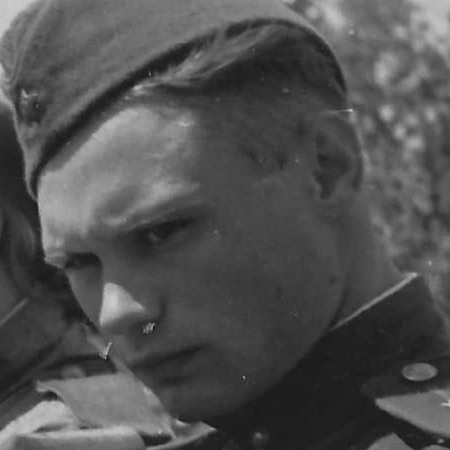
\includegraphics[height=80pt]{tatiana.jpg}
\end{multicols}
\end{center}
\noindent\makebox[\linewidth]{\rule{\textwidth}{0.4pt}}
%ATTRIBUTS
\subsection*{Attributs}
\begin{center}
    \begin{tabular}{c|c|c|c|c}
        \textbf{Autorité} & \textbf{Chance} & \textbf{Combativité} & \textbf{Endurance} & \textbf{Sang-froid} \\
        4 & 2 & 4 & 4 & 2\\

    \end{tabular}
\end{center}
\begin{tabular}{m{0.4\columnwidth} m{0.4\columnwidth}}
     \textbf{Stress :} & \textbf{Points de progression :}
\end{tabular}\\
\noindent\makebox[\linewidth]{\rule{\textwidth}{0.4pt}}
%COMPETENCES
\subsection*{Compétences}
\begin{tabular}{p{0.4 \textwidth}| r || p{0.4 \textwidth}| r|}
Athlétisme & 3 &Conduite : & 0\\
Connaissances Techniques : mécanique& 2 &Connaissances Techniques : & 0\\
Conviction & 0 &Couverture& 4\\
Discipline & 0 &Infiltration& 2\\
Interrogation & 0 & Labeur& 3\\
Logistique & 2 & Maintenance : armes d'épaules& 3\\
Maintenance: mécanique & 2& Mêlée& 2\\
Observation & 3 & Opération : & 0\\
Opération : & 0 & Orientation& 2\\
Premiers soins & 0 & Survie& 3\\
Tactiques & 3 & Tir : arme d'épaule& 4\\
Tir : jet & 3 & Tir : arme de poing & 1\\
\end{tabular}\\
\noindent\makebox[\linewidth]{\rule{\textwidth}{0.4pt}}
\subsection*{Matériel}
uniforme militaire, gourde, sac à dos, rations pour deux jours,\\
pistolet-mitrailleur ppsh-41 (épaule, portée 75/300, barrage, combat rapproché, automatique 75) \\
pelle affûtée(poing, combat rapproché), casque (défense 6+)\\
cocktails molotovs (jet, portée 20/30, incendiaire, perforant 2, AP)\\
revolver Nagant M1895 (poing, portée 45, combat rapproché)\\
\noindent\makebox[\linewidth]{\rule{\textwidth}{0.4pt}}

\subsection*{Notes}
Ancienne étudiante à l'université de mécanique de Leningrad, elle s'est engagée dans l'armée rouge après avoir été évacuée de sa ville natale, présentement assiégée par les fascistes. Elle se bat pour leur rendre la monnaie de leur pièce, et mène souvent l'attaque. Elle a rejoint la 13ème lors de la reformation récente. Sa camarade lui fournit un soutient à distance quand elle part à l'assaut.

%FICHE 2
\newpage
\ttfamily
\begin{center}
%SECTION GROUPEE : état civil
\section*{Dossier de personnel}
\begin{multicols}{3}
\textbf{Nom :} Piotr Ilyich Bukarin\\
\textbf{Genre :} Homme\\
\textbf{Date de naissance :} 17.11.1923\\
\textbf{Camarade :} Ivan Nomokonov(labeur, athlétisme, mêlée)\\
\textbf{Traits particuliers :}\\
\columnbreak
\textbf{Grade et spécialité :}infirmier \\
\textbf{Yeux :} Bleus\\
\textbf{Cheveux :} Blonds\\
\textbf{Taille :} 1m70\\
\columnbreak
\includegraphics[height=80pt]{piotr.jpg}
\end{multicols}
\end{center}
\noindent\makebox[\linewidth]{\rule{\textwidth}{0.4pt}}
%ATTRIBUTS
\subsection*{Attributs}
\begin{center}
    \begin{tabular}{c|c|c|c|c}
        \textbf{Autorité} & \textbf{Chance} & \textbf{Combativité} & \textbf{Endurance} & \textbf{Sang-froid} \\
         2&4 &2 &5 &3\\

    \end{tabular}
\end{center}
\begin{tabular}{m{0.4\columnwidth} m{0.4\columnwidth}}
     \textbf{Stress :} & \textbf{Points de progression :}
\end{tabular}\\
\noindent\makebox[\linewidth]{\rule{\textwidth}{0.4pt}}
%COMPETENCES
\subsection*{Compétences}
\begin{tabular}{p{0.4 \textwidth}| r || p{0.4 \textwidth}| r|}
Athlétisme & 3 &Conduite : & 0\\
Connaissances Techniques : & 0 &Connaissances Techniques : & 0\\
Conviction & 1 &Couverture& 4\\
Discipline & 0 &Infiltration& 2\\
Interrogation & 1 & Labeur& 2\\
Logistique & 3 & Maintenance : armes d'épaules& 2\\
Maintenance: & 0& Mêlée& 2\\
Observation & 3 & Opération : & 0\\
Opération : & 0 & Orientation& 2\\
Premiers soins & 3 & Survie& 2\\
Tactiques & 3 & Tir : arme d'épaule& 2\\
Tir : jet & 3 & Tir : arme de poing & 3\\
\end{tabular}\\
\noindent\makebox[\linewidth]{\rule{\textwidth}{0.4pt}}
%MATERIEL ET NOTES
\subsection*{Matériel}
uniforme militaire, gourde, sac à dos, rations pour deux jours,\\
fusil mosin-nagant (épaule, portée 300/800, gênante, perforante (1)) \\
couteau de combat(poing, combat rapproché)\\
grenades RGD-33 (jet, portée 20/30, zone, combat rapproché)\\
Civière simple\\
\noindent\makebox[\linewidth]{\rule{\textwidth}{0.4pt}}

\subsection*{Notes}
Ayant travaillé en tant qu'assistant dans un cabinet médical à Arkangelsk, Piotr a reçu une rapide formation aux premiers secours et nommé infirmier. Il se bat pour défendre sa terre natale, menacée par les envahisseurs qui ravagent le pays. Avec son camarade, ils transportent les blessés vers l'arrière et essaient de les stabiliser. Il a rejoint l'unité récemment; il était auparavant attaché à une unité d'artillerie depuis la fin 1941.
%FICHE 3
\newpage
\ttfamily
\begin{center}
%SECTION GROUPEE : état civil
\section*{Dossier de personnel}
\begin{multicols}{3}
\textbf{Nom :} Mikhail Ivanovich Tulayev\\
\textbf{Genre :}Homme\\
\textbf{Date de naissance :} 27.01.1905\\
\textbf{Camarade :} Fyodor Okhlokov(tactique, conviction, athlétisme)\\
\textbf{Traits particuliers :}\\
\columnbreak
\textbf{Grade et spécialité :} Sergent\\
\textbf{Yeux : bruns}\\
\textbf{Cheveux : noirs}\\
\textbf{Taille : 1.70}\\
\columnbreak
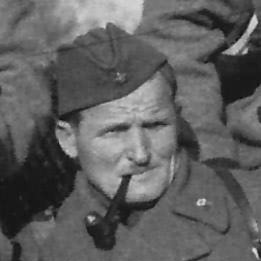
\includegraphics[height=80pt]{mikhail.jpg}
\end{multicols}
\end{center}
\noindent\makebox[\linewidth]{\rule{\textwidth}{0.4pt}}
%ATTRIBUTS
\subsection*{Attributs}
\begin{center}
    \begin{tabular}{c|c|c|c|c}
        \textbf{Autorité} & \textbf{Chance} & \textbf{Combativité} & \textbf{Endurance} & \textbf{Sang-froid} \\
         4&2 &2 &5 &3\\

    \end{tabular}
\end{center}
\begin{tabular}{m{0.4\columnwidth} m{0.4\columnwidth}}
     \textbf{Stress :} & \textbf{Points de progression :}
\end{tabular}\\
\noindent\makebox[\linewidth]{\rule{\textwidth}{0.4pt}}
%COMPETENCES
\subsection*{Compétences}
\begin{tabular}{p{0.4 \textwidth}| r || p{0.4 \textwidth}| r|}
Athlétisme &2 &Conduite : & 0\\
Connaissances Techniques : & 0 &Connaissances Techniques : & 0\\
Conviction & 2 &Couverture& 3\\
Discipline & 3 &Infiltration& 2\\
Interrogation & 2& Labeur& 1\\
Logistique & 2& Maintenance : armes d'épaule & 2 \\
Maintenance: & 0 & Mêlée& 2\\
Observation & 3 & Opération : & 0\\
Opération : & 0 & Orientation& 2\\
Premiers soins & 1 & Survie& 3\\
Tactiques & 5 & Tir : arme d'épaule& 3\\
Tir : arme de poing & 2& Tir : jet & 3\\
\end{tabular}\\
\noindent\makebox[\linewidth]{\rule{\textwidth}{0.4pt}}
%MATERIEL ET NOTES
\subsection*{Matériel}
uniforme militaire, gourde, sac à dos, rations pour deux jours,montre et carte,\\
pistolet-mitrailleur ppsh-41 (épaule, portée 75/300, barrage, combat rapproché, automatique 75) \\
couteau de combat(poing, combat rapproché)\\
2 grenades RGD-33 (jet, portée 20/30, zone, combat rapproché)\\
revolver Nagant M1895 (poing, portée 25/75, combat rapproché)\\
\noindent\makebox[\linewidth]{\rule{\textwidth}{0.4pt}}
\subsection*{Notes}
Un des vétérans de la division, puisqu'elle était encore quand il l'a rejoint la première brigade aéroportée. Il suit fidèlement son commandant, le brigadier Rodimtsev depuis le début de la guerre. C'est un soldat de métier, ayant rejoint plutôt jeune l'armée rouge pour faire oublier ses origines de Kulak (paysans riches, persécutés par Staline).
%FICHE 4
\newpage
\ttfamily
\begin{center}
%SECTION GROUPEE : état civil
\section*{Dossier de personnel}
\begin{multicols}{3}
\textbf{Nom :} Maria Muhametqyzy Surkova\\
\textbf{Genre :}Femme\\
\textbf{Date de naissance :} 25.10.1925\\
\textbf{Camarade :} Alexandra Samusenko (couverture, infiltration, observation)\\
\textbf{Traits particuliers :}cicatrice à la joue gauche\\
\columnbreak
\textbf{Grade et spécialité :} sniper\\
\textbf{Yeux : bruns}\\
\textbf{Cheveux : noirs}\\
\textbf{Taille : 1.65}\\
\columnbreak
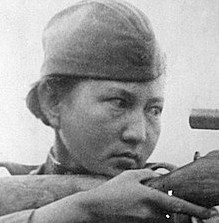
\includegraphics[height=80pt]{Maria.jpg}
\end{multicols}
\end{center}
\noindent\makebox[\linewidth]{\rule{\textwidth}{0.4pt}}
%ATTRIBUTS
\subsection*{Attributs}
\begin{center}
    \begin{tabular}{c|c|c|c|c}
        \textbf{Autorité} & \textbf{Chance} & \textbf{Combativité} & \textbf{Endurance} & \textbf{Sang-froid} \\
         2&3 &2 &5 &4\\

    \end{tabular}
\end{center}
\begin{tabular}{m{0.4\columnwidth} m{0.4\columnwidth}}
     \textbf{Stress :} & \textbf{Points de progression :}
\end{tabular}\\
\noindent\makebox[\linewidth]{\rule{\textwidth}{0.4pt}}
%COMPETENCES
\subsection*{Compétences}
\begin{tabular}{p{0.4 \textwidth}| r || p{0.4 \textwidth}| r|}
Athlétisme &4 &Conduite : & 0\\
Connaissances Techniques : & 0 &Connaissances Techniques : & 0\\
Conviction & 0 &Couverture& 5\\
Discipline & 3 &Infiltration& 4\\
Interrogation & 0& Labeur& 1\\
Logistique & 2& Maintenance : armes d'épaule & 1 \\
Maintenance: lunette& 2 & Mêlée& 1\\
Observation & 4 & Opération : & 0\\
Opération : & 0 & Orientation& 3\\
Premiers soins & 0 & Survie& 1\\
Tactiques & 2 & Tir : arme d'épaule& 7\\
Tir : arme de poing & 2& Tir : jet & 0\\
\end{tabular}\\
\noindent\makebox[\linewidth]{\rule{\textwidth}{0.4pt}}
%MATERIEL ET NOTES
\subsection*{Matériel}
uniforme militaire, gourde, sac à dos, rations pour deux jours,\\
cape de camouflage, jumelles \\
couteau de combat(poing, combat rapproché)\\
fusil mosin-nagant avec lunette(épaule, portée 500/800, gênante, perforante 1, précise, déploiement 1), revolver Nagant M1895 (poing, portée 25/75, combat rapproché)\\
\noindent\makebox[\linewidth]{\rule{\textwidth}{0.4pt}}
\subsection*{Notes}
La jeune Khazakh s'est engagée à la déclaration de guerre contre son pays, par conviction : elle a foi dans le rêve communiste d'égalité et de modernité. Elle a combattu près de Moscou au cours de l'hiver 1942 avant d'être assignée à la 13ème division de la garde. Sa camarade repère ses cibles, qu'elle abat de son fusil.
%FICHE 5
\newpage
\ttfamily
\begin{center}
%SECTION GROUPEE : état civil
\section*{Dossier de personnel}
\begin{multicols}{3}
\textbf{Nom : Kliment Alexsandrevich Frolov}\\
\textbf{Genre :}\\\textbf{Date de naissance : 07.08.1917}\\
\textbf{Camarade :Akim Lagutin}(labeur, maintenance, logistique)\\
\textbf{Traits particuliers :}lunettes de vue\\
\columnbreak
\textbf{Grade et spécialité :}artilleur \\
\textbf{Yeux :} bleus\\
\textbf{Cheveux :}rasés\\
\textbf{Taille : }1m65\\
\columnbreak
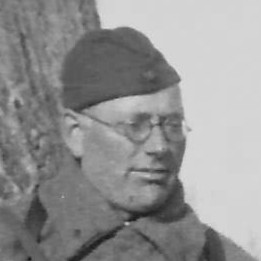
\includegraphics[height=80pt]{Kliment.jpg}
\end{multicols}
\end{center}
\noindent\makebox[\linewidth]{\rule{\textwidth}{0.4pt}}
%ATTRIBUTS
\subsection*{Attributs}
\begin{center}
    \begin{tabular}{c|c|c|c|c}
        \textbf{Autorité} & \textbf{Chance} & \textbf{Combativité} & \textbf{Endurance} & \textbf{Sang-froid} \\
         2&2 &4 &4 &4\\

    \end{tabular}
\end{center}
\begin{tabular}{m{0.4\columnwidth} m{0.4\columnwidth}}
     \textbf{Stress :} & \textbf{Points de progression :}
\end{tabular}\\
\noindent\makebox[\linewidth]{\rule{\textwidth}{0.4pt}}
%COMPETENCES
\subsection*{Compétences}
\begin{tabular}{p{0.4 \textwidth}| r || p{0.4 \textwidth}| r|}
Athlétisme & 3&Conduite : & 0\\
Connaissances Techniques : bricolage& 3 &Connaissances Techniques : & 0\\
Conviction & 1 &Couverture& 3\\
Discipline & 0 &Infiltration& 2\\
Interrogation &0 & Labeur& 2\\
Logistique &2 & Maintenance : arme d'épaule& 1\\
Maintenance: arme de soutien &1 & Mêlée& 1\\
Observation &0 & Opération : & 0\\
Premiers soins &0 & Orientation& 2\\
 Tactiques &3 & Survie& 3\\
Tir : arme de poing &2 & Tir : arme d'épaule & 3\\
Tir : soutien &4 & Tir : jet& 2\\
\end{tabular}\\
\noindent\makebox[\linewidth]{\rule{\textwidth}{0.4pt}}
%MATERIEL ET NOTES
\subsection*{Matériel}
uniforme militaire, gourde, sac à dos, rations pour deux jours, casque (défense 6)\\
cocktails molotovs (jet, portée 20/30, incendiaire, perforant 2, AP), pelle affûtée(poing, combat rapproché), revolver Nagant M1895 (poing, portée 25/75, combat rapproché)\\
fusil mosin-nagant (épaule, portée 500, gênante, perforante 1) \\
mitrailleuse Maxim avec bouclier (soutien, portée 500/1200, barrage, zone, perforante(1), encombrante, défense 5+, automatique 500)\\
\noindent\makebox[\linewidth]{\rule{\textwidth}{0.4pt}}
\subsection*{Notes}
Kliment est une des dernières recrues de la division, s'étant engagé il y a trois mois, après avoir entendu les horreurs qu'ils infligeaient aux paysans de l'ouest. Avec lui, beaucoup de ses camarades ouvriers s'engagèrent, et il connaît de cette époque une dizaine d'homme du 1er bataillon. Son camarade veille au bon ravitaillement en munition de sa maxim, et aide à la tracter.
\rmfamily
\chapter*{Annexes}
\section*{Glossaire}
\begin{multicols}{2}\setlength{\columnsep}{0.5cm}
\setlength{\columnseprule}{0.5pt}
\begin{description}
\item[MJ] Maître du Jeu, joueur ayant un rôle spécial, celui de gérer les obstacles que doivent affronter les personnages au cours de l'histoire, ainsi que les personnages non-joueurs.
  \item[Tension] Réserve de points utilisée pour représenter la tension dramatique de l'histoire, et le danger général contre les PJs.
  \item[Menace] Une menace est un composant adverse lors d'un combat, un groupe d'adversaires, une unité ennemie lointaine ou un danger du terrain par exemple.
  \item[PJ] Personnage joueur, les personnages incarnés par les personnes autour de la table, sauf ceux du MJ.
  \item[PNJ]Personnage non-joueur, les personnages incarnés par le MJ, avec lesquels les PJs interagissent.
  \item[d6] Dé à six faces, dé standard utilisé dans \nomjeu
  \item[SR] Seuil de Réussite, difficulté à battre pour accomplir une action avec succès.
  \item[JdR] Jeux de Rôle(s) : type de jeu permettant à un groupe de joueurs de créer l'histoire de différents personnages, en imaginant cette histoire au fur et à mesure, dans le cadre de règles plus ou moins rigides.
  \item[\diminutif] \nomjeu
\end{description}
\end{multicols}

\section*{Inspirations}
\begin{multicols}{2}\setlength{\columnsep}{0.5cm}
\setlength{\columnseprule}{0.5pt}
\subsection*{Films}
\begin{itemize}
    \item Il faut sauver le soldat Ryan
    \item Dunkerque
    \item Full Metal Jacket
    \item Lettres d'Iwo Jima
    \item Fury
    \item Rogue One: a Star Wars story
    \item Band of Brothers
\end{itemize}

\subsection*{Lectures}
\begin{itemize}
    \item Le choix du courage
    \item Lazarre en guerre
    \item Les fantomes de Gaunt
    \end{itemize}
\end{multicols}
\section*{Documentaires et sources historiques}
\begin{itemize}
    \item facingstalingrad.com
    \item Military History Visualised (youtube)
    \item Stalingrad, Anthony Beevor
\end{itemize}

%FICHE DE PERSONNAGE
\newpage
\ttfamily

%SECTION GROUPEE : état civil
\section*{Dossier de personnel}
%\begin{flushright}
%\includegraphics[height=100pt]{placeholder.png}
%\end{flushright}



\begin{multicols}{3}
\textbf{Nom :}\\
\textbf{Genre :}\\\textbf{Date de naissance :}\\
\textbf{Camarade :}\\
\textbf{Traits particuliers :}\\
\columnbreak
\textbf{Grade et spécialité :} \\
\textbf{Yeux :}\\
\textbf{Cheveux :}\\
\textbf{Taille :}\\
\columnbreak
\includegraphics[height=80pt]{placeholder.png}
\end{multicols}
\noindent\makebox[\linewidth]{\rule{\textwidth}{0.4pt}}


%ATTRIBUTS
\subsection*{Attributs}
\begin{center}
    \begin{tabular}{c|c|c|c|c}
        \textbf{Autorité} & \textbf{Chance} & \textbf{Combativité} & \textbf{Endurance} & \textbf{Sang-froid} \\
         & & & &\\

    \end{tabular}
\end{center}
\begin{center}
    \begin{tabular}{m{0.4\columnwidth} m{0.4\columnwidth}}
     \textbf{Stress :} & \textbf{Points de progression :}
\end{tabular}
\end{center}
\noindent\makebox[\linewidth]{\rule{\textwidth}{0.4pt}}
%COMPETENCES
\subsection*{Compétences}

\begin{tabular}{p{0.4 \textwidth}| r || p{0.4 \textwidth}| r|}
Athlétisme & &Conduite : & {}\\
Connaissances Techniques : &  &Connaissances Techniques : & {}\\
Conviction &  &Couverture& {}\\
Discipline &  &Infiltration& {}\\
Interrogation & & Labeur& {}\\
Logistique & & Maintenance : & {}\\
Maintenance: & & Mêlée& {}\\
Observation & & Opération : & {}\\
Opération : & & Orientation& {}\\
Premiers soins & & Survie& {}\\
Tactiques & & Tir : & {}\\
Tir : & & Tir : & {}\\

\end{tabular}\\
\noindent\makebox[\linewidth]{\rule{\textwidth}{0.4pt}}
%MATERIEL ET NOTES
\subsection*{Matériel}
\begin{tabular}{c}
     \\ \\ \\ \\ \\ \\ \\ \\
\end{tabular}

\noindent\makebox[\linewidth]{\rule{\textwidth}{0.4pt}}


\subsection*{Notes}
%idées en vrac:
%xp en récompense des échecs, ou des actions du MJ, plus que des actions réussies, permet de récompenser toutes les actions des joueurs, ne pas avoir de moments purement négatifs lors d'une session.
\rmfamily
\end{document}
